\title{Word2vecを用いた文章構造の解析手法}
\author{プロジェクトマネジメントコース\\
ソフトウェア開発管理グループ\\
矢吹研究室\\
1442069\\
須山武弘}
\date{}
\begin{document}
\maketitle

%\noindent
□□□□□□□□□■□□□□□□□□□■□□□□□□□□□■□□□□□□□□□■
□□□□□□□□□■□□□□□□□□□■□□□□□□□□□■□□□□□□□□□■
□□□□□□□□□■□□□□□□□□□■□□□□□□□□□■□□□□□□□□□■
□□□□□□□□□■□□□□□□□□□■□□□□□□□□□■□□□□□□□□□■
□□□□□□□□□■□□□□□□□□□■□□□□□□□□□■□□□□□□□□□■
□□□□□□□□□■□□□□□□□□□■□□□□□□□□□■□□□□□□□□□■
□□□□□□□□□■□□□□□□□□□■□□□□□□□□□■□□□□□□□□□■
□□□□□□□□□■□□□□□□□□□■□□□□□□□□□■□□□□□□□□□■
□□□□□□□□□■□□□□□□□□□■□□□□□□□□□■□□□□□□□□□■
□□□□□□□□□■□□□□□□□□□■□□□□□□□□□■□□□□□□□□□■
□□□□□□□□□■□□□□□□□□□■□□□□□□□□□■□□□□□□□□□■
□□□□□□□□□■□□□□□□□□□■□□□□□□□□□■□□□□□□□□□■
□□□□□□□□□■□□□□□□□□□■□□□□□□□□□■□□□□□□□□□■
□□□□□□□□□■□□□□□□□□□■□□□□□□□□□■□□□□□□□□□■
□□□□□□□□□■□□□□□□□□□■□□□□□□□□□■□□□□□□□□□■
□□□□□□□□□■□□□□□□□□□■□□□□□□□□□■□□□□□□□□□■
□□□□□□□□□■□□□□□□□□□■□□□□□□□□□■□□□□□□□□□■
□□□□□□□□□■□□□□□□□□□■□□□□□□□□□■□□□□□□□□□■
□□□□□□□□□■□□□□□□□□□■□□□□□□□□□■□□□□□□□□□■
□□□□□□□□□■□□□□□□□□□■□□□□□□□□□■□□□□□□□□□■
□□□□□□□□□■□□□□□□□□□■□□□□□□□□□■□□□□□□□□□■
□□□□□□□□□■□□□□□□□□□■□□□□□□□□□■□□□□□□□□□■
□□□□□□□□□■□□□□□□□□□■□□□□□□□□□■□□□□□□□□□■
□□□□□□□□□■□□□□□□□□□■□□□□□□□□□■□□□□□□□□□■
□□□□□□□□□■□□□□□□□□□■□□□□□□□□□■□□□□□□□□□■
□□□□□□□□□■□□□□□□□□□■□□□□□□□□□■□□□□□□□□□■
□□□□□□□□□■□□□□□□□□□■□□□□□□□□□■□□□□□□□□□■
□□□□□□□□□■□□□□□□□□□■□□□□□□□□□■□□□□□□□□□■
□□□□□□□□□■□□□□□□□□□■□□□□□□□□□■□□□□□□□□□■
□□□□□□□□□■□□□□□□□□□■□□□□□□□□□■□□□□□□□□□■
□□□□□□□□□■□□□□□□□□□■□□□□□□□□□■□□□□□□□□□■
□□□□□□□□□■□□□□□□□□□■□□□□□□□□□■□□□□□□□□□■
□□□□□□□□□■□□□□□□□□□■□□□□□□□□□■□□□□□□□□□■
□□□□□□□□□■□□□□□□□□□■□□□□□□□□□■□□□□□□□□□■
□□□□□□□□□■□□□□□□□□□■□□□□□□□□□■□□□□□□□□□■
□□□□□□□□□■□□□□□□□□□■□□□□□□□□□■□□□□□□□□□■
□□□□□□□□□■□□□□□□□□□■□□□□□□□□□■□□□□□□□□□■
□□□□□□□□□■□□□□□□□□□■□□□□□□□□□■□□□□□□□□□■
□□□□□□□□□■□□□□□□□□□■□□□□□□□□□■□□□□□□□□□■
■■■■■■■■■■■■■■■■■■■■■■■■■■■■■■■■■■■■■■■■
□□□□□□□□□■□□□□□□□□□■□□□□□□□□□■□□□□□□□□□■%文字数チェック用

\tableofcontents%目次
%1章序論
\chapter{序論}
レポートや論文を書く際には,読みやすく,論理的な文章を書くことが大切である.論理的文章を書くための書き方として,世界で標準的なパラグラフ・ライティング(Paragraph writing)がある.パラグラフ・ライティングは,英語文章の一般的スタイルであり,序論,本論,結論の3部構成となっている.序論でトピックとなる文が示され,本論は序論に続く支持文となり,最後に結論で文章をまとめる.冒頭にトピックとなる文章を示すと伝えたいことが明確になり,速読が可能となったり,内容の理解が深まるなど多数のメリットがある.

言語を定量的に表すツールとして,Word2vecがある.Word2vecは,単語をベクトルへ変換することができるため,文章の話題の方向性を解析し,文章作成の補助ができるのではないかと仮説を立て,本研究に取り組んだ.
\newpage

%2章背景
\chapter{背景}
%2.1章
\section{本研究の全体的背景}
近年,コンピュータは人間と対話するようになってきている.ソフトバンク社の開発した,感情認識ヒューマノイドロボットのPepperを始めとするロボットや,Amazon社の発売するAIスピーカーEcho,身近な存在ではスマートフォンの音声認識システムもそうである.また,これから大きく普及するであろうIoT(Internet of Things:モノをインターネットに繋ぐ技術)技術を用いた様々なものにも音声認識システムは搭載されるであろう.このことから,コンピュータは人間が自然に発する言語である自然言語を理解し,処理,出力することが要求されている.
このような,コンピュータにおける自然言語処理の必要性が高まっていることに注目し,コンピュータと自然言語でなにか研究はできないかと考えた.
Word2vecを用いてコンピュータに処理をさせ,自然言語を数値化し,文書構造を解析させることを考えた.
\newpage

%2.2章
\section{自然言語}
自然言語とは,人間が日常の意思疎通のために用いられ,自然に発せられる言語のことである.人間が自然に発する言語ということもで,人それぞれの出身やできごとなどの文化的背景などが絡み,曖昧な表現が含まれる.そのため,プログラム言語などの数学的言語とは違い,曖昧さを含んでいる自然言語は直接コンピュータが認識することはできない.このことから,コンピュータへ自然言語を認識させるには自然言語処理が必要である.
\begin{figure}[htb]
\centering
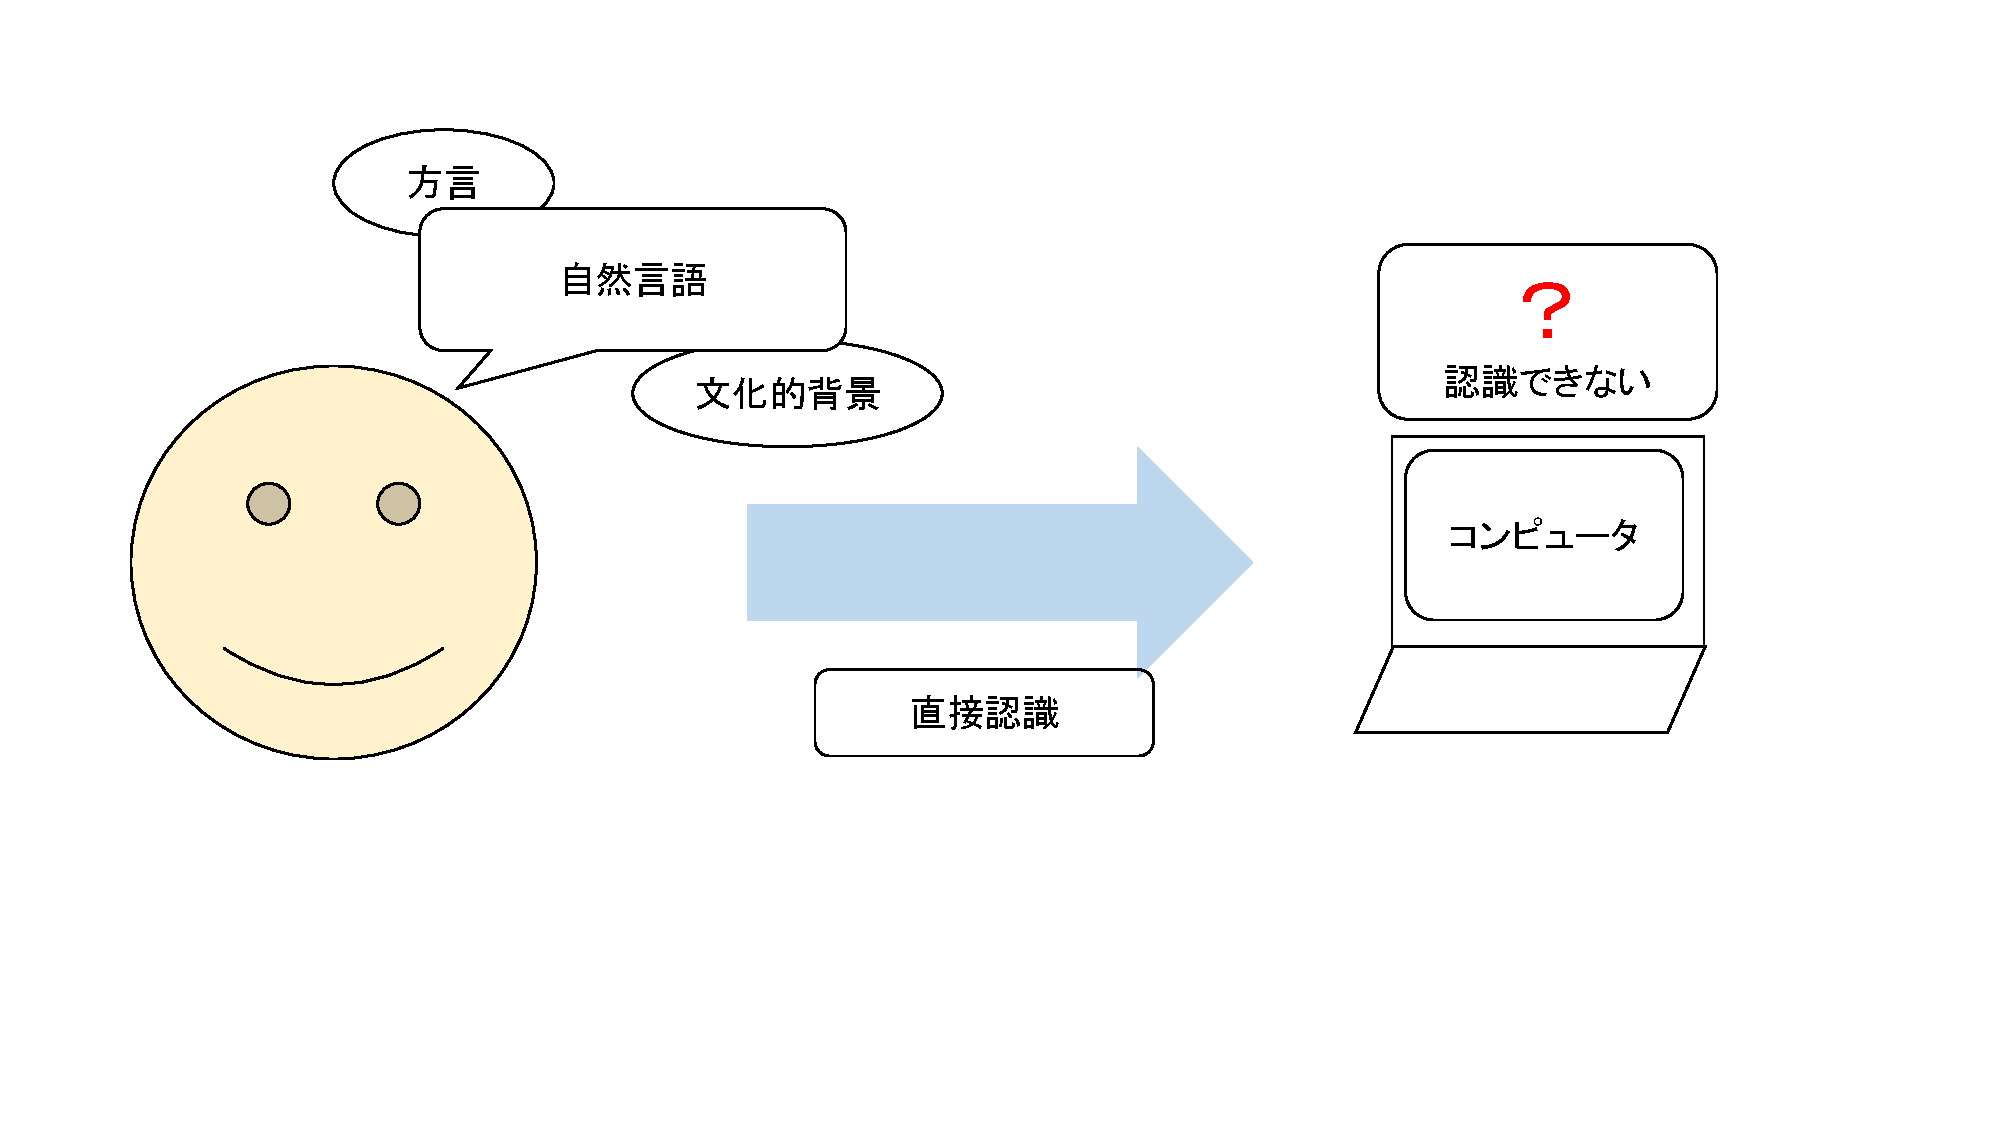
\includegraphics[width=10cm]{2-1.pdf}
\caption{自然言語は直接認識できない}\label{2-1}
\end{figure}
\newpage

%2.3章
\section{自然言語処理}
自然言語処理とは,前述した自然言語をコンピュータへ認識させるために行う処理のことである.
\begin{figure}[htb]
\centering
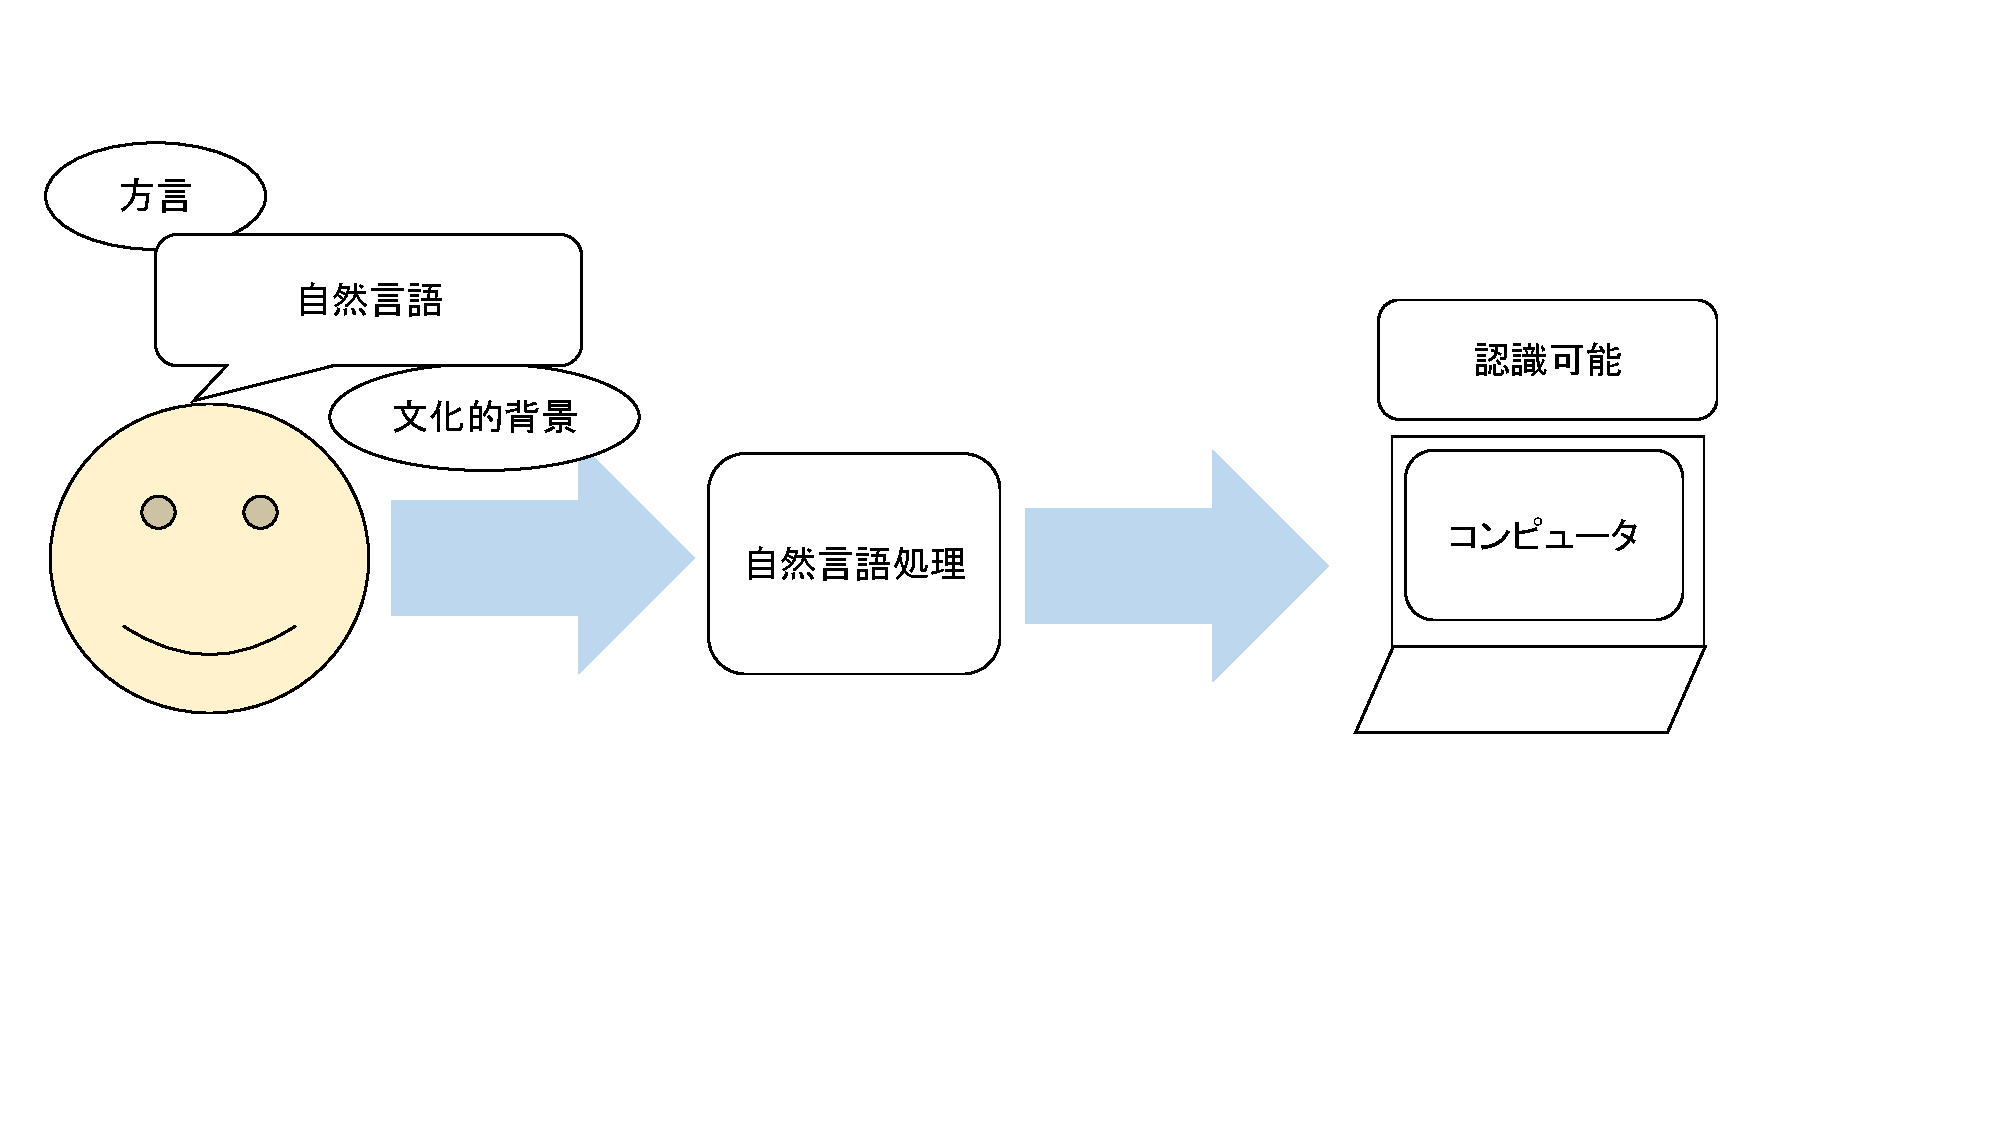
\includegraphics[width=10cm]{2-2.pdf}
\caption{コンピュータへの認識}\label{2-2}
\end{figure}
\newpage

%2.4章
\section{Word2vecについて}
本研究で用いるWord2vecは,テキスト処理を行うニューラルネットワークのことである.コーパスを入力すると,単語の特徴量ベクトルが出力される.つまり,テキストを数値化することができる.

また,Word2vecは類似後のベクトルをベクトル空間にグループ化することができるので,数値に基づいて類似性を判断することができる.
%2.4.1章
\subsection{コーパスとは}
コーパスとは,自然言語処理の研究に用いるため,自然言語の文章を構造化し,大規模に集積したものである.Word2vecでは,MeCabを利用し,形態素解析を行ったあと,コーパスを作成することができるが,Wikipediaなど,大量のデータを利用してコーパスを作成するのには非常に時間がかかる.
\newpage

%3章目的
\chapter{目的}
Word2vecを用いて文字列である文章をベクトルへ変換し,定量的に文章構造を解析することでパラグラフ・ライティングができているかを調査する.
\newpage

%4章手法
\chapter{手法}
%4.1章
\section{本研究全体の流れ}
以下の手順で研究を進めた.
\begin{enumerate}
 \item 仮想環境の導入.
 \item Word2vec環境構築.
 \item 形態素解析(MeCabwo使用)
 \item 日本語 Wikipedia エンティティベクトルのコーパスを使用し,Word2vecによって文章をベクトルへ変換.
 \item Rの導入.
 \item 多数の文章で主成分分析.
\end{enumerate}
\newpage

%4.2章
\section{Linuxについて}
Linuxとは,WindowsやMacOSと同じOS(オペレーティング・システム)のことである.Linuxは,Unixが源流のオープンソースOSである.オープンソースなので,無料で使え,改変可能なプログラムである.

Linuxを使うにあたって,様々な特徴がある.
\begin{enumerate}
 \item 無料である.
 \item オープンソースのため,改変が可能である.
 \item プログラムを動かす環境として優れている.
 \item 低スペックなコンピュータでも動作可能である
\end{enumerate}
\newpage

%4.3章
\section{使用・インストールするツール}
本研究では仮想環境を用いて研究を行ったため,仮想環境の構築手法を記す.
%4.3.1章
\subsection{chocolatey}
今回,環境構築に必要なものをインストールするにあたり,chocolateyをインストールする.これは,必要なソフトがまとめてインストールが可能であるため,これを利用しソフトウェアをインストールする.

chocolatreyの大まかなインストール手順は以下の通りである.
\begin{enumerate}
 \item chocolateyのWebページへ行き,インストールコマンドをコピーする.
 \item 管理者権限のあるコマンドプロンプト(PowerShell)を起動し,ペーストする.
 \item インストールするもののコマンドを入力する.
\end{enumerate}

「chocolatey」とweb検索をするか,

https://chocolatey.org/

のURLへアクセスすれば,chocolateyの公式ページへ飛ぶことができる.

\begin{figure}[htb]
\centering
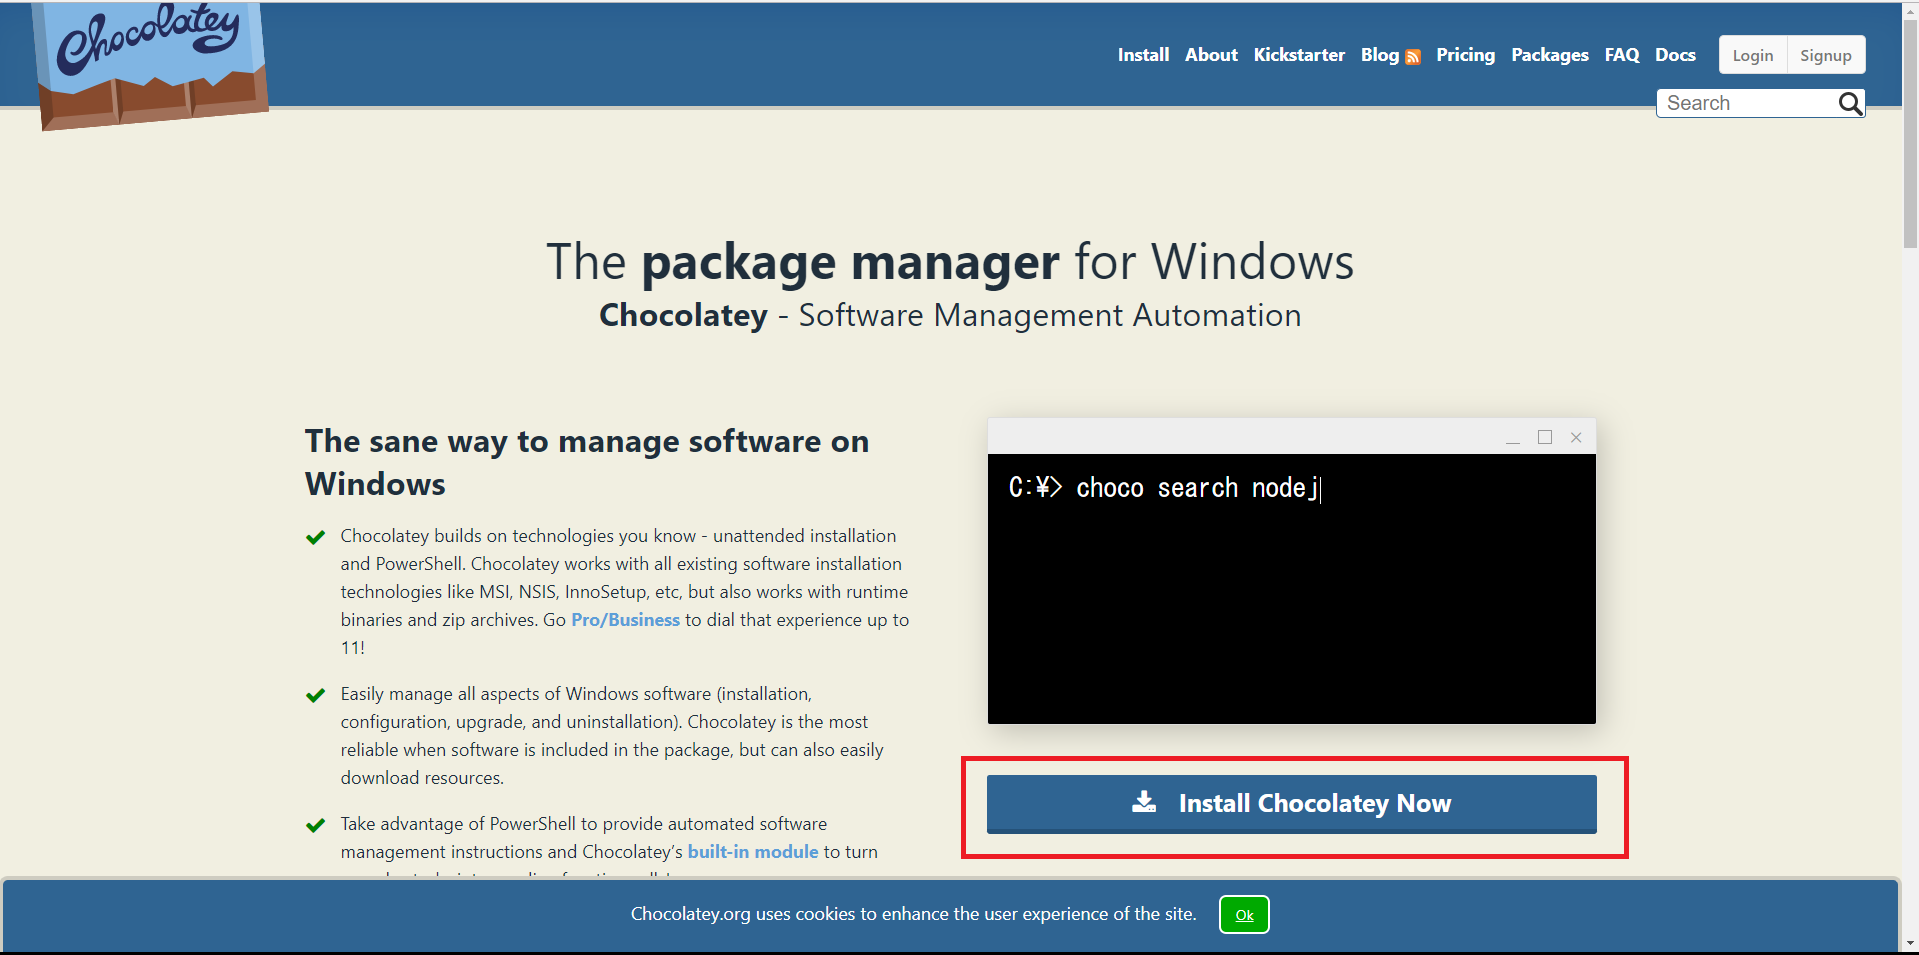
\includegraphics[width=13cm]{4-1.png}
\caption{chocolateyHP}\label{4-1}
\end{figure}
上図の赤枠部へアクセスすると,インストール画面へ遷移する.
\newpage

インストールページへ遷移したら,少し下へスクロールをする.そうすると,赤枠部のようなテキストが見えてくる.

コマンドプロンプトを利用する場合は赤枠部上,PowerShellを利用している場合は下のテキストをコピーし,管理者権限のあるコマンドプロンプトにペーストする.
\begin{figure}[htb]
\centering
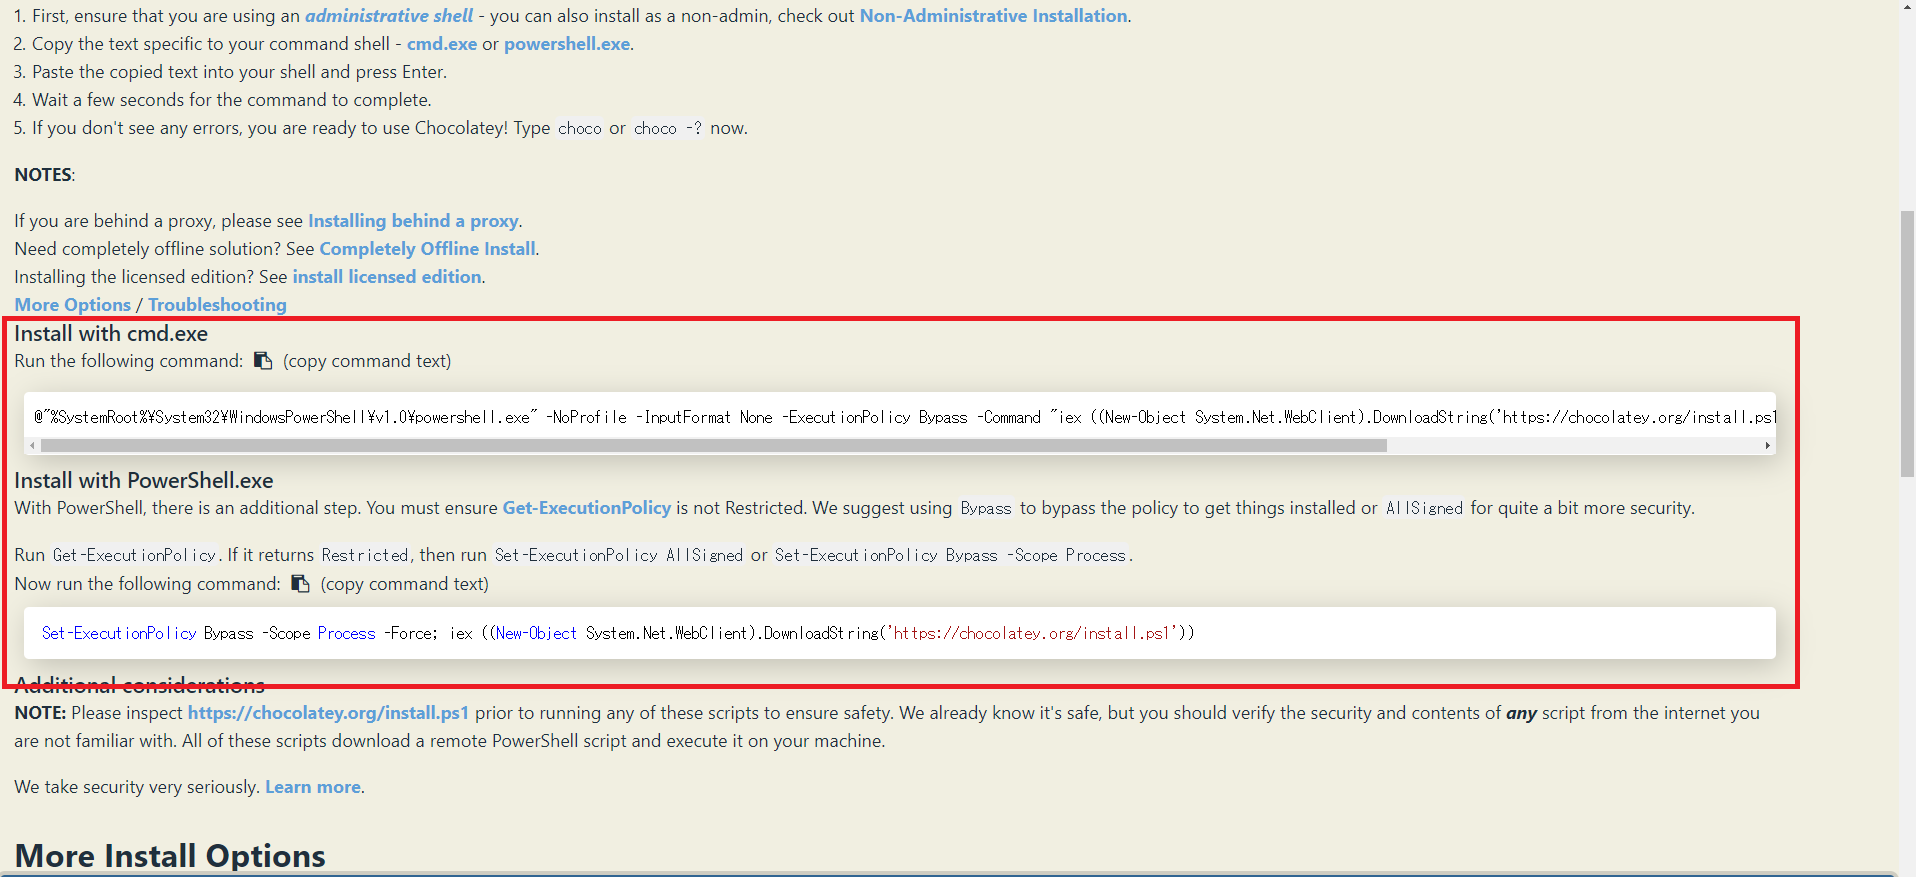
\includegraphics[width=13cm]{4-2.png}
\caption{chocolateyインストールページ}\label{4-2}
\end{figure}
\newpage

管理者権限のあるコマンドプロンプト(PowerShell)を起動する.ここで,管理者権限のないコマンドプロンプトを開いてしまわぬよう注意すること.

先程のコピーしてきたコマンドをペーストし,以下のようになれば成功である.
\begin{figure}[htb]
\centering
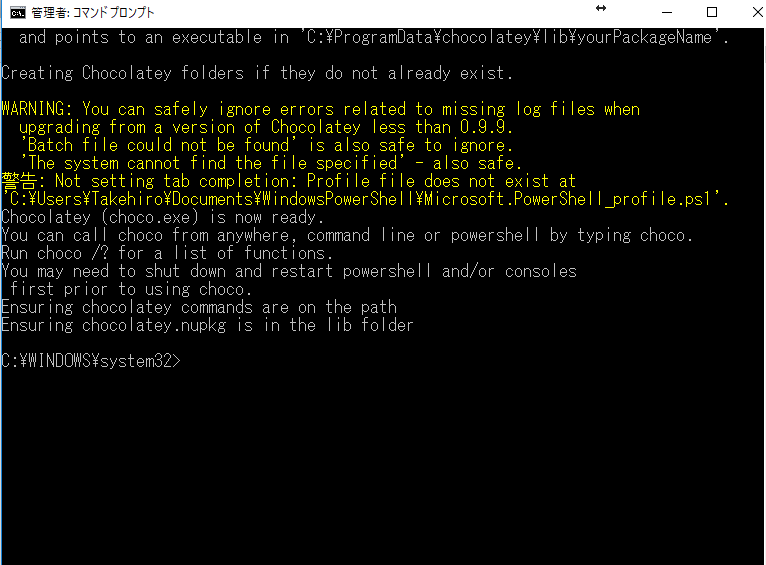
\includegraphics[width=13cm]{4-3.png}
\caption{chocolateyインストール}\label{4-3}
\end{figure}
\newpage


他にインストールをしたいものがある場合は,以下のページにアクセスするとインストールできるパッケージの一覧が見れる.インストールしたいパッケージのコマンドを管理者用コマンドプロンプトへ入力するとインストールできる.

https://chocolatey.org/packages

\begin{figure}[htb]
\centering
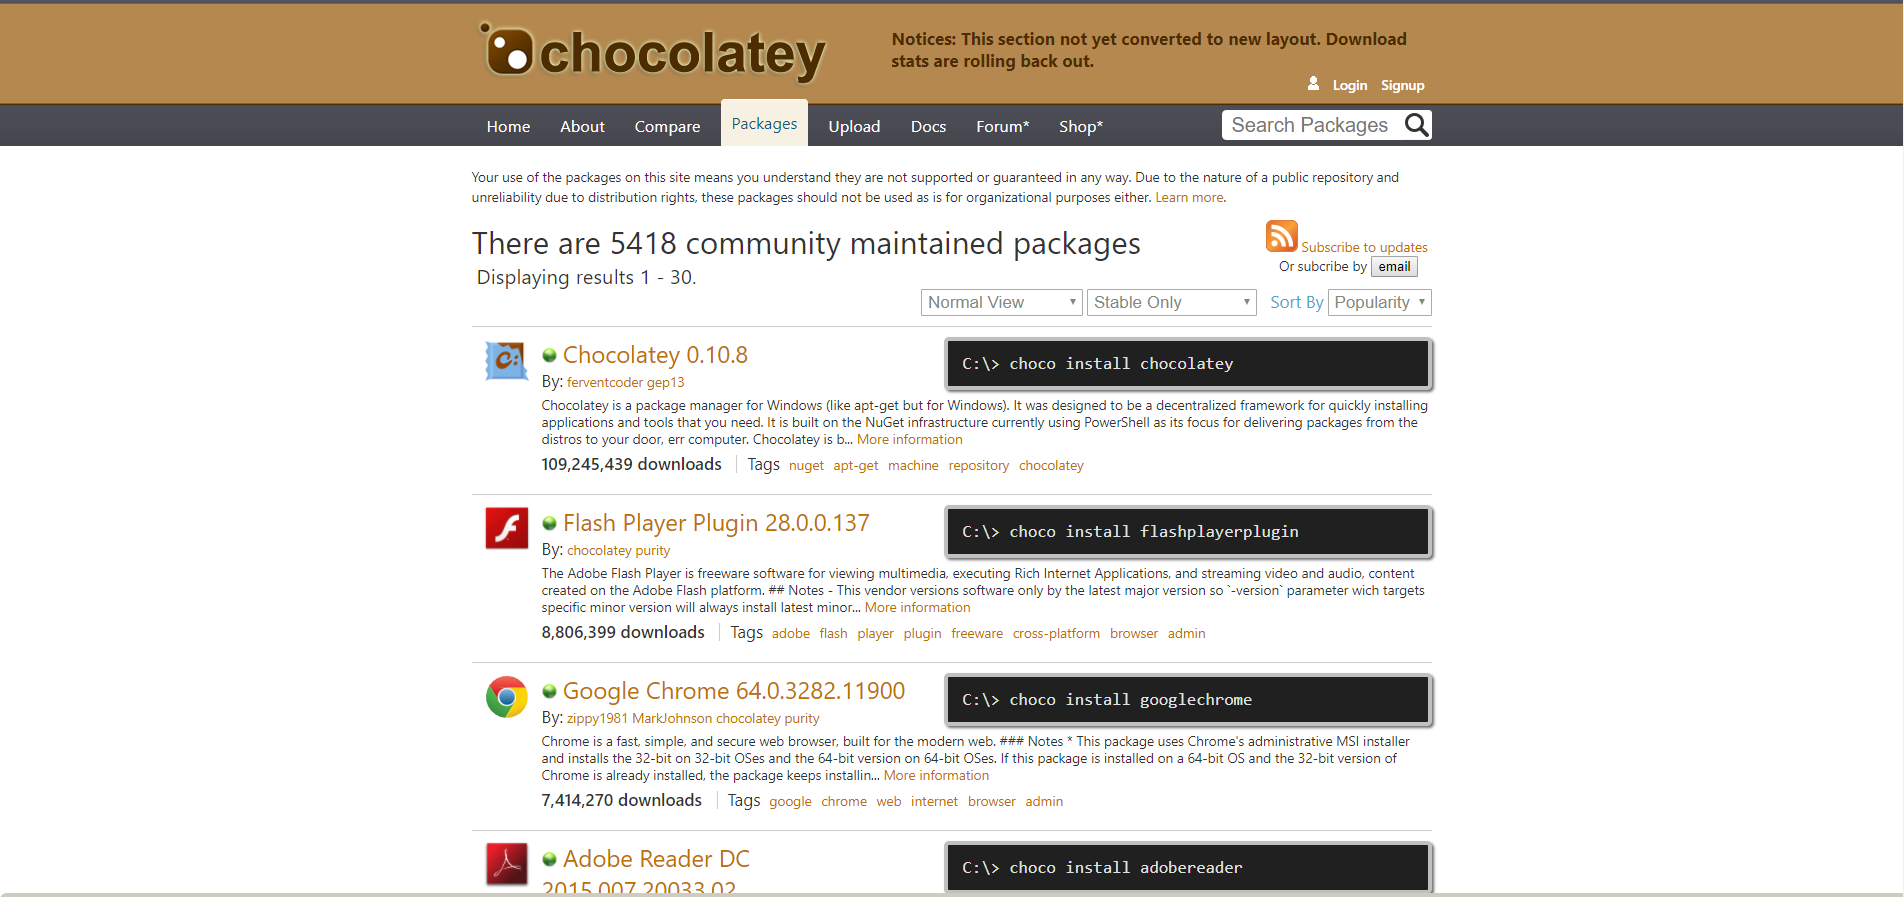
\includegraphics[width=13cm]{4-4.png}
\caption{chocolateパッケージ}\label{4-4}
\end{figure}
\newpage
%4.3.2章
\subsection{VirtualBox}
本研究では,Windows上でLinux環境を構築するためにVirtualBoxを使用する.本来,LinuxOSを扱いたいが,WindowsOSのマシンの為,VirtualBoxを使用し,使用しているマシン上に仮想的なマシンを作成し,別のOSをインストール・実行できるようにする.

\begin{figure}[htb]
\centering
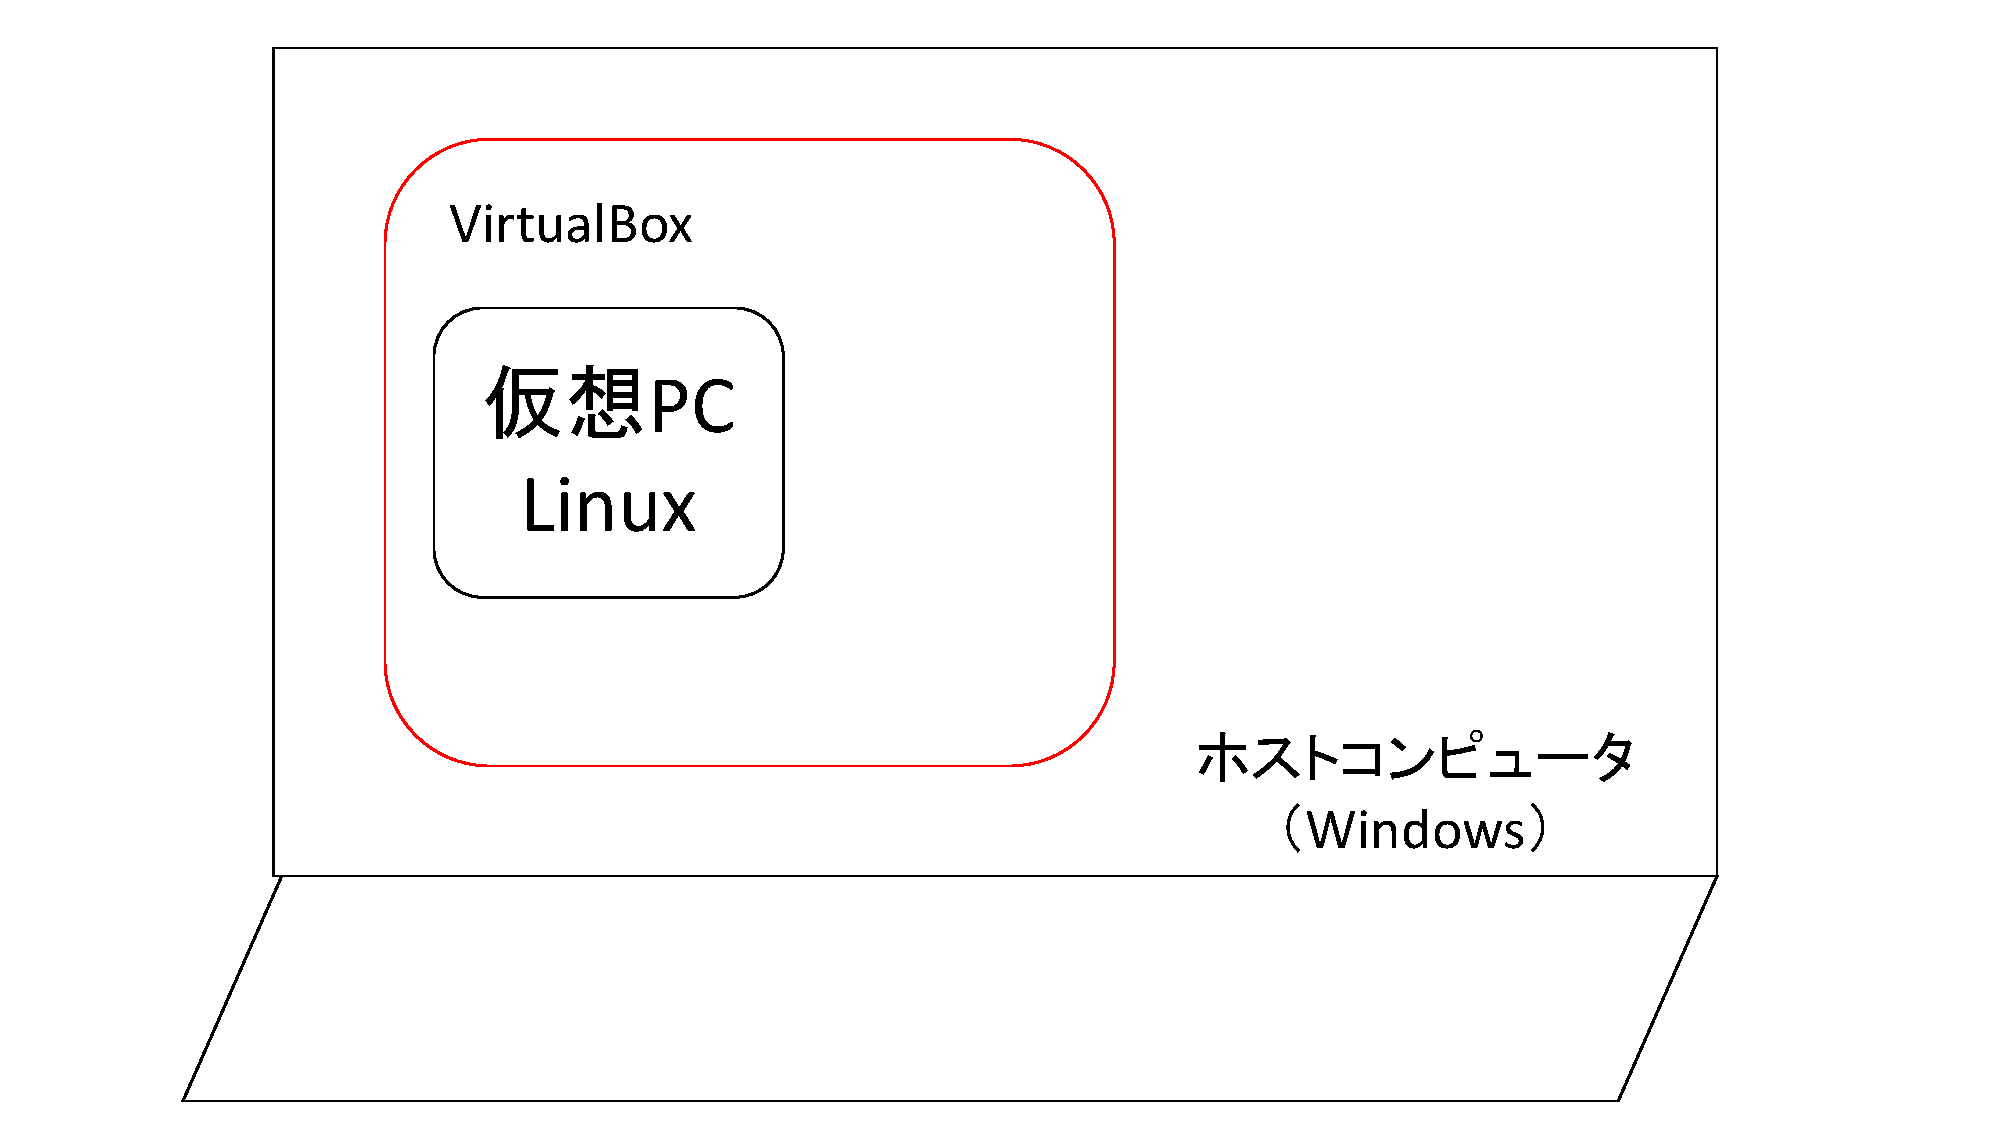
\includegraphics[width=13cm]{4-5.pdf}
\caption{VirtualBox 概要}\label{4-5}
\end{figure}
\newpage

VirtualBoxはコンピュータ上で直接動作している通常のOSにとってはアプリケーションの一つであり,ほかのソフトと同じように起動することができるものである.起動すると仮想的なマシンが構築され,元のOSとは独立に別のOSを起動することができる.VirtualBoxが実行されているOSをホストOS,VirtualBox上で実行されているOSをゲストOSという.

元は独立系のソフトウェア企業が開発・販売していた製品だったが,開発元がSun Microsystems社に買収され,その後同社がOracle社に買収されたため,Oracle社が開発元となり,正式名称も「Oracle VM VirtualBox」となっている.さらに,VirtualBox本体はGPLに基づいたオープンソースソフトウェアとして公開され,だれでも自由に入手・利用・改変・再配布などが行える.

VirtualBoxを使う上での注意点として,現時点でのVirtualBoxは仮想メモリをサポートしていないため,実メモリ以上のメモリを仮想PCが使用することはできない.仮想メモリを使うと動作が遅くなるため,仮想PCには実メモリ以内のサイズを割り当てる.そのため,仮想PCを1台だけ起動するのであれば問題ないが,複数の仮想PCを同時に起動させる場合これがネックになってしまう.同時起動させる全ての仮想PCのメモリサイズの合計が実メモリのサイズを超えないようにする.そのため,VurtualBoxをインストールするPCには多くのメモリが必要で,最低4GB以上のPCを使うようにするべきである.本研究に用いる際もかそうPCのメモリは2GBでは足りないので,注意が必要である.
\newpage

次に,chocolateyを使用したVirtualBoxのインストール方法を説明する.

下図のように

choco install virtualbox

とコマンドを入力すると,インストールすることができる.

\begin{figure}[htb]
\centering
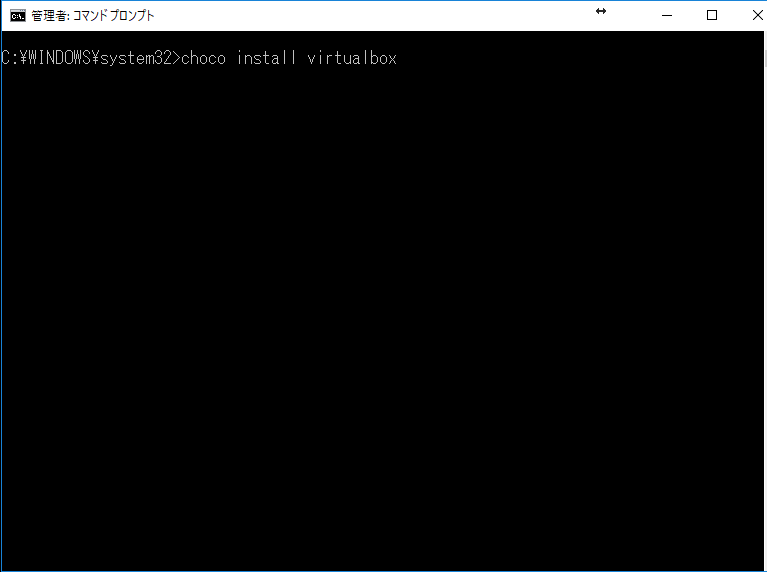
\includegraphics[width=13cm]{4-6.png}
\caption{chocolatey VirtualBoxのインストール}\label{4-6}
\end{figure}
\newpage

実際にVirtualBoxを起動し,図4.7のようになれば成功である.
\begin{figure}[htb]
\centering
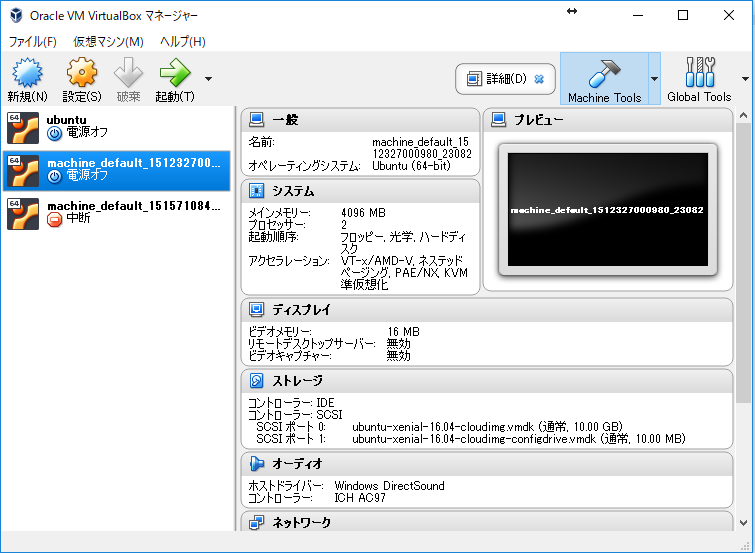
\includegraphics[width=13cm]{4-7.png}
\caption{chocolatey VirtualBoxのインストール}\label{4-7}
\end{figure}
\newpage

\subsubsection{VirtualBoxの用語}

\subsubsection{ホストマシン}

物理的に存在するコンピュータのこと.

\subsubsection{ホストOS}

ホストマシンにインストールされているOSのこと.VirtualBoxはホストOSにインストールされる.

\subsubsection{バーチャルマシン(仮想マシン)}

VirtualBoxが作成する論理的なマシンのこと.ゲストマシンに割り当てるために,VirtualBoxがホストマシンのコンピュータ資源(CPUやメモリ,HDD等)の一部を仮想化する.ホストマシンの資源を使い切らない限り,ゲストマシンを複数作成したり,多重起動させることができる.

\subsubsection{ゲストOS(仮想OS)}

ゲストマシンにインストールされるOSのこと.

\subsubsection{仮想ディスク}

ゲストマシンが使用する仮想のハードディスクのこと.バーチャルマシンからはこれを物理ディスクとして扱うことができる.仮想ディスクの実態はホストマシン内にファイルとして存在する.
\newpage

%4.3.3章
\subsection{Vagrant}
Vagrantとは,仮想環境を簡単に構築・管理することができるツールである.Vagrantを使用することにより,仮想マシンの設定や作成などが容易にできる.

Vagrantを用いるにあたって,様々な利点がある.
\begin{enumerate}
 \item コマンド一つで仮想マシンを作成することができる.
 \item ホストマシンの環境に依存せずに開発やテストができる.
 \item Vagrantfileに構成を記述できるので,環境構築が楽になる.
 \end{enumerate}
\newpage

\subsubsection{Vagrantのインストール}
Vagrantはchocolateyのコマンドでインストールすることができる.

コマンドは以下の通りである.管理者権限のあるコマンドプロンプトに

choco install -y vagrant 

と入力し,実行する.

\begin{figure}[htb]
\centering
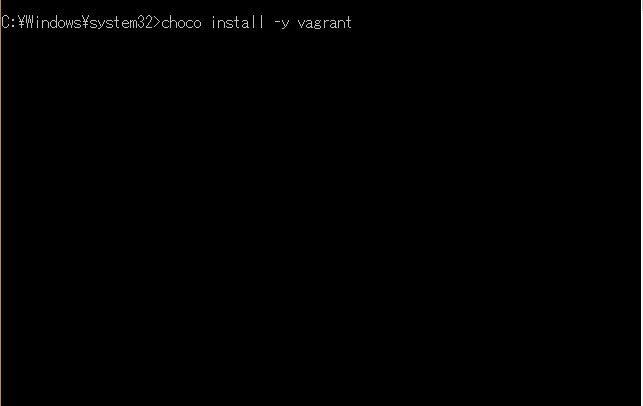
\includegraphics[width=13cm]{4-8.png}
\caption{chocolatey Vagrantのインストール}\label{4-8}
\end{figure}
\newpage

図4.9のようになればインストール成功である.
\begin{figure}[htb]
\centering
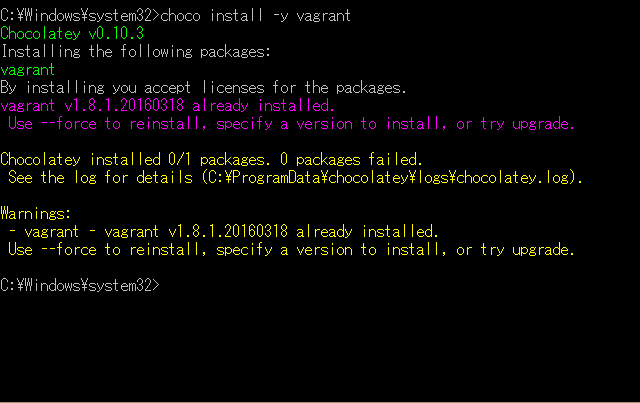
\includegraphics[width=13cm]{4-9.png}
\caption{chocolatey Vagrantのインストール完了}\label{4-9}
\end{figure}
\newpage

\subsubsection{Vagrant起動の仕方}
コマンドプロンプトを起動し,”/Vagnrat/machine”までディレクトリを変更する.

やり方は以下の通りである.

”cd /vagrant/machine”

と入力し,実行する.cdとは,チェンジディレクトリの意味である.
\begin{figure}[htb]
\centering
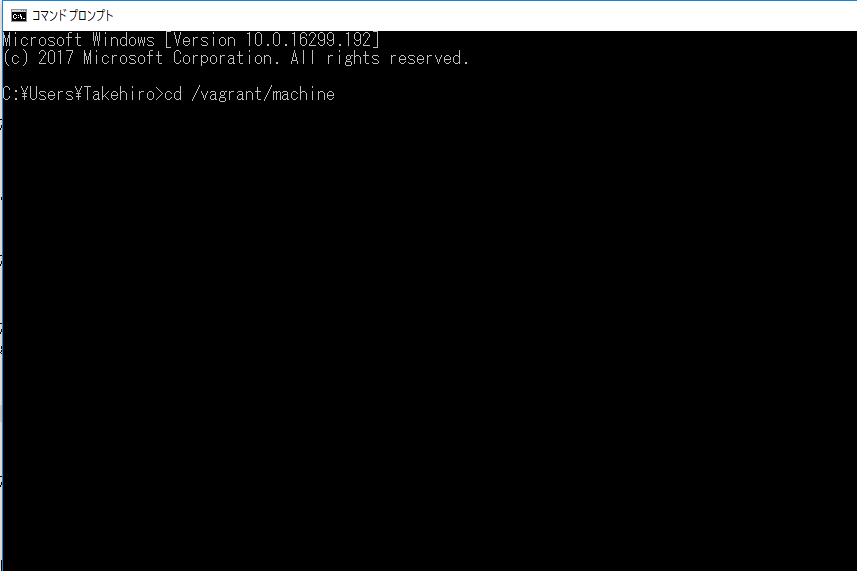
\includegraphics[width=13cm]{4-10.png}
\caption{Vagrant起動 ディレクトリ変更}\label{4-10}
\end{figure}
\newpage

以下のようになればディレクトリの変更に成功している.

\begin{figure}[htb]
\centering
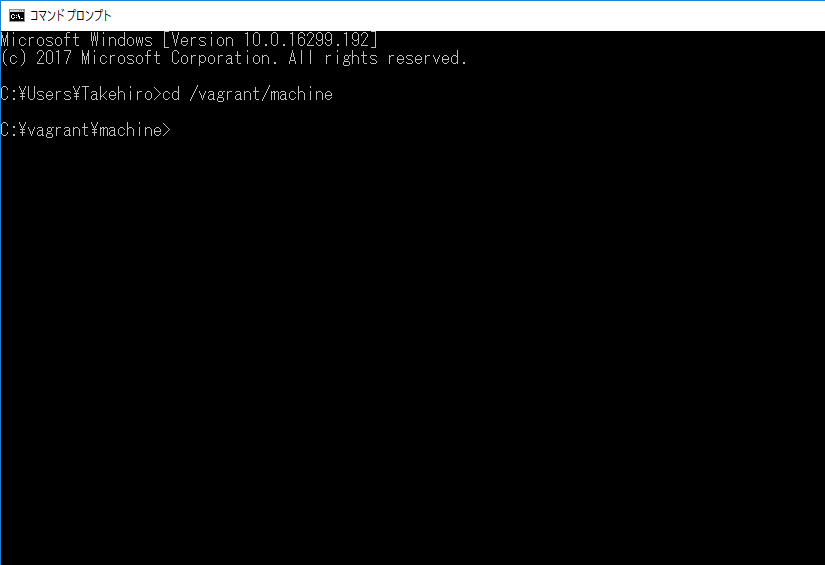
\includegraphics[width=13cm]{4-11.png}
\caption{Vagrant起動 ディレクトリ変更完了}\label{4-11}
\end{figure}
\newpage

ディレクトリの変更が済んだら,マシンの起動コマンドを入力する.
起動コマンドは,”vagrant up”である.
\begin{figure}[htb]
\centering
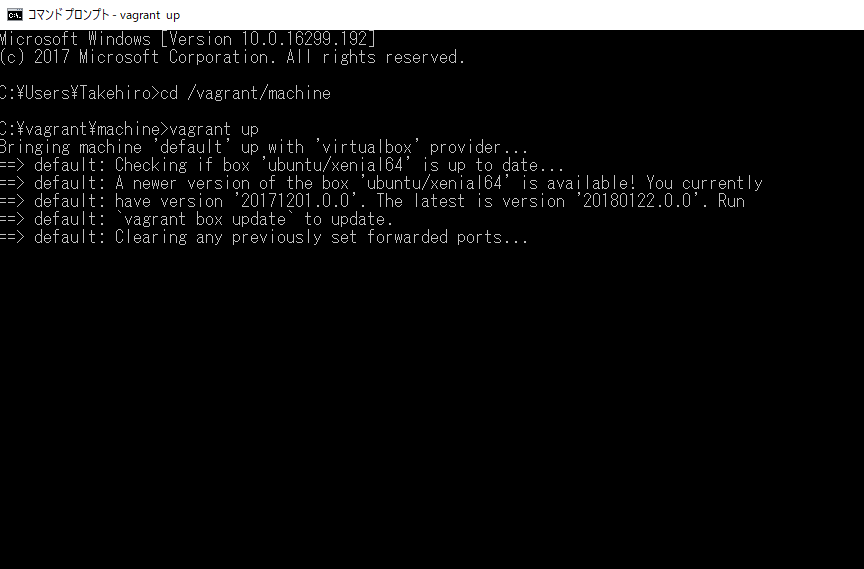
\includegraphics[width=13cm]{4-12.png}
\caption{Vagrant起動}\label{4-12}
\end{figure}
\newpage

以下のようになれば起動完了である.なお,初回起動には時間がかかるので暫く待つ必要がある.
\begin{figure}[htb]
\centering
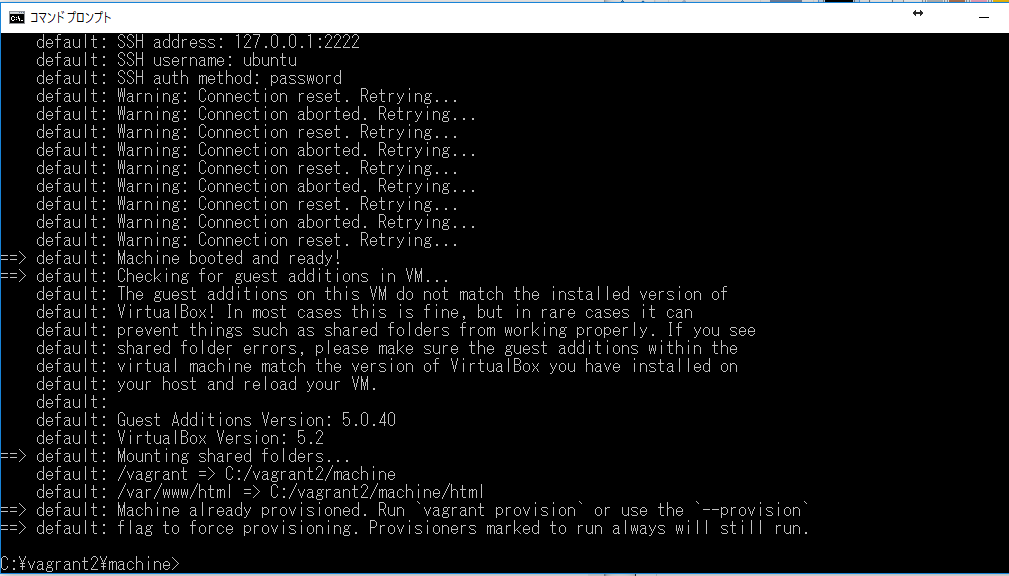
\includegraphics[width=13cm]{4-13.png}
\caption{Vagrant起動完了}\label{4-13}
\end{figure}
\newpage

仮想マシンへのログイン方法は下記の通りである.

vagrant upを実行したところへ

”vagrant ssh”

と入力する.以下のようになれば成功である.
\begin{figure}[htb]
\centering
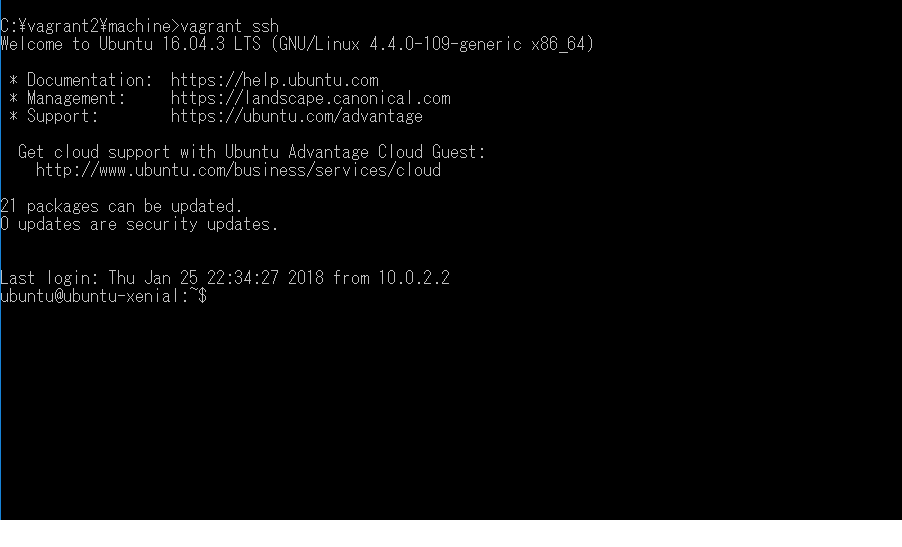
\includegraphics[width=13cm]{4-14.png}
\caption{VagrantSSH}\label{4-14}
\end{figure}
\newpage

ログアウト方法は,「Ctrl + D」でログアウトする.以下のようになれば成功である.
\begin{figure}[htb]
\centering
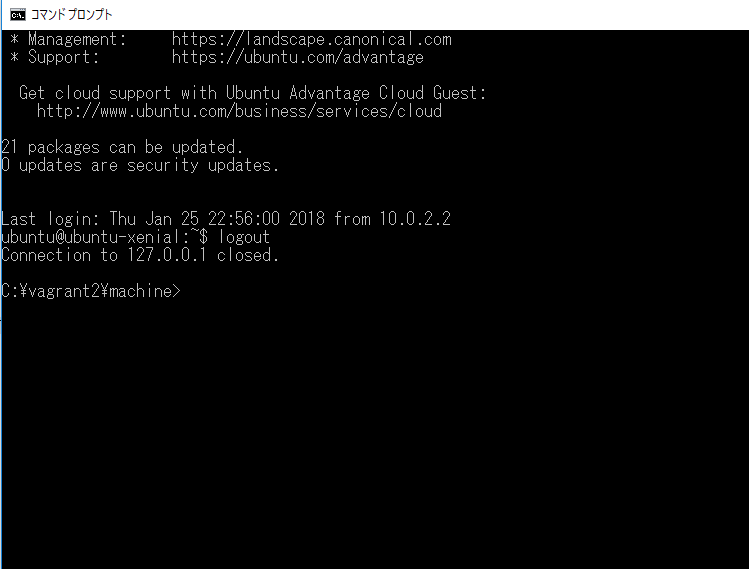
\includegraphics[width=13cm]{4-15.png}
\caption{Vagrantログアウト}\label{4-15}
\end{figure}
\newpage

だが,ログアウトしただけで仮想マシンの電源は切れていない.

そこで,電源を切るコマンドを下記の通り実行し,図4.16のようになれば成功である.

”vagrant halt”

\begin{figure}[htb]
\centering
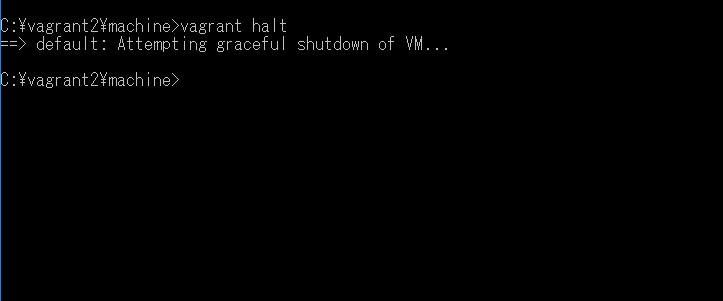
\includegraphics[width=13cm]{4-16.png}
\caption{Vagrant シャットダウン}\label{4-16}
\end{figure}
\newpage

\subsubsection{Vagrantコマンド}

\subsubsection{vagrant up}
仮想マシンの起動を行う.

\subsubsection{vagrant ssh}
仮想マシンの再起動を行う.

\subsubsection{vagrant halt}
仮想マシンの停止を行う.

\subsubsection{vagrant destroy}
仮想マシンの削除を行う.

\subsubsection{vagrant ssh}
仮想マシンにログイン.
\newpage

%4.4章
\section{環境構築}
本研究では,VirtualBox,Vagrantを使用し,仮想環境を構築した.
これまでの説明は,本研究に用いるツールの基本的インストール方法や,基本的知識である.ここからは,本研究で実際に用いた環境設定を書く.なお,chocolatey,VirtualBox,Vagrantがインストール済みであることが前提となっている.

本研究においては,矢吹研究室公式の仮想マシンを使用する.

まず,管理者権限でないコマンドプロンプトを起動し,Guest Additionの更新,ディスクサイズの変更を簡易化するためのプラグインを導入する.
\newpage

それぞれ,以下のようになれば成功である.

\begin{figure}[htb]
\centering
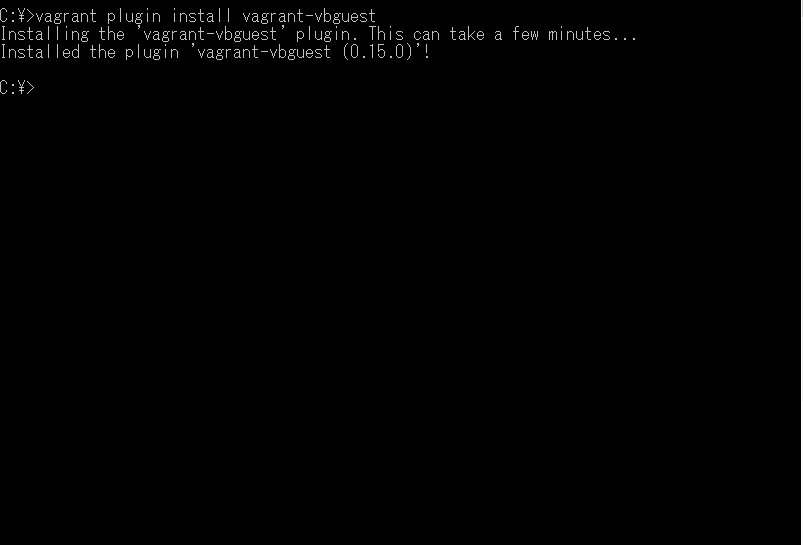
\includegraphics[width=11cm]{4-17.png}
\caption{Guest Additionの更新}\label{4-17}
\end{figure}

\begin{figure}[htb]
\centering
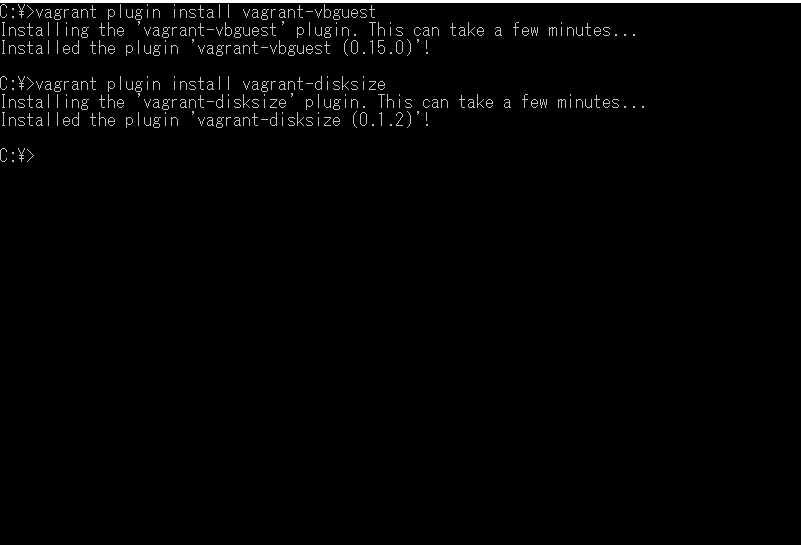
\includegraphics[width=11cm]{4-18.png}
\caption{ディスクサイズの変更を簡易化するためのプラグインを導入}\label{4-18}
\end{figure}
\newpage

次に仮想マシンを用意する.先ほどと同じく,管理者でないコマンドプロンプトに以下のコマンドを実行する.コマンドの意味も下記の通りである.

cd /

ルートディレクトリへ変更.

mkdir vagrant

vagrantというフォルダを作成.

以下のように何も出てこなければ成功である.念のため,図4.20のように作成されているか確認すると良い.

\begin{figure}[htb]
\centering
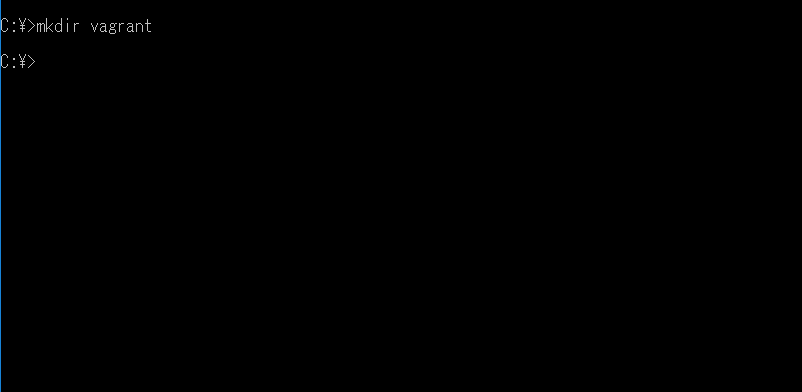
\includegraphics[width=11cm]{4-19.png}
\caption{フォルダ作成}\label{4-19}
\end{figure}

\begin{figure}[htb]
\centering
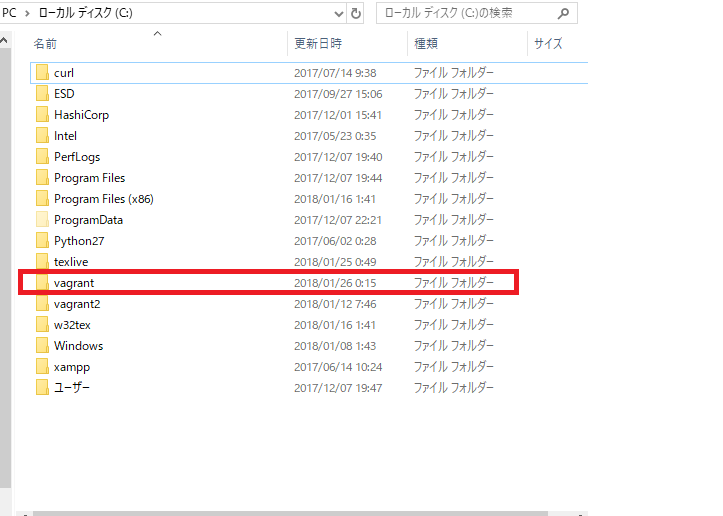
\includegraphics[width=11cm]{4-20.png}
\caption{フォルダ作成 確認}\label{4-20}
\end{figure}
\newpage

cd /vagrant


先ほど作成したvagrantというフォルダ内へ移動


git clone https://github.com/yabukilab/machine.git


矢吹研究室公式マシンのgithubとクローンする.

以下のようになればクローン成功である.
\begin{figure}[htb]
\centering
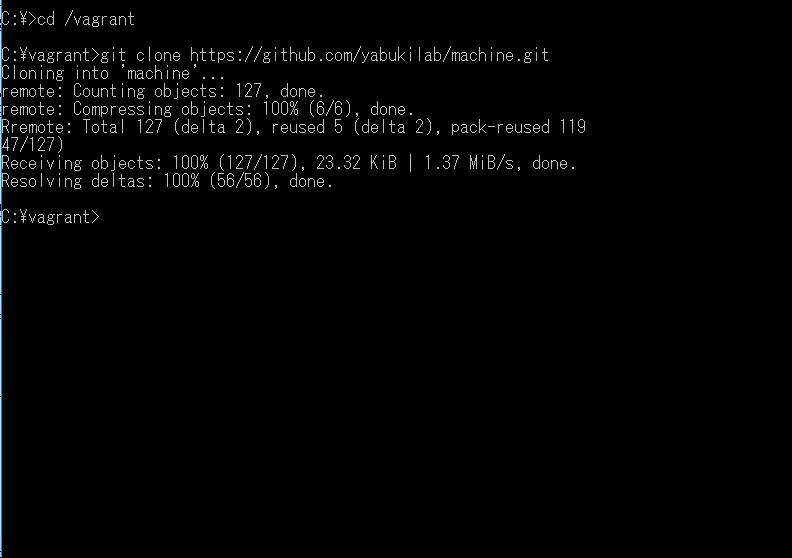
\includegraphics[width=13cm]{4-21.png}
\caption{矢吹件公式マシン クローン}\label{4-21}
\end{figure}
\newpage

次に,下記コマンドでmachineディレクトリへ移動する.

cd machine

本研究では,メモリの容量が不足してしまうため,仮想マシンの起動をする前にVagrantfileの設定を変える必要がある.メモリ容量の変更方法は下記のとおりである.

C:/vagrant/machine の中にVagrantfileというファイルが存在する.このファイルをテキストエディタで開く.

\begin{figure}[htb]
\centering
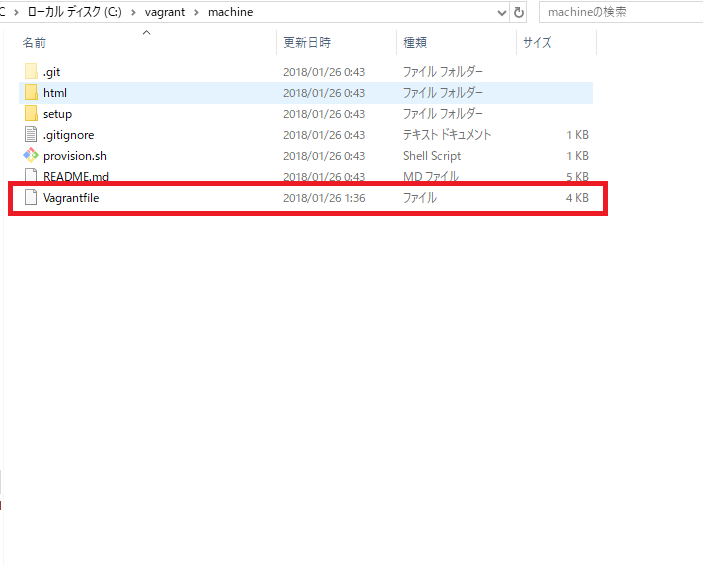
\includegraphics[width=13cm]{4-22.png}
\caption{Vagrantfile}\label{4-22}
\end{figure}
\newpage

テキストエディタで開いたら,59行目のメモリ容量を2GB以上に増やす.
\begin{figure}[htb]
\centering
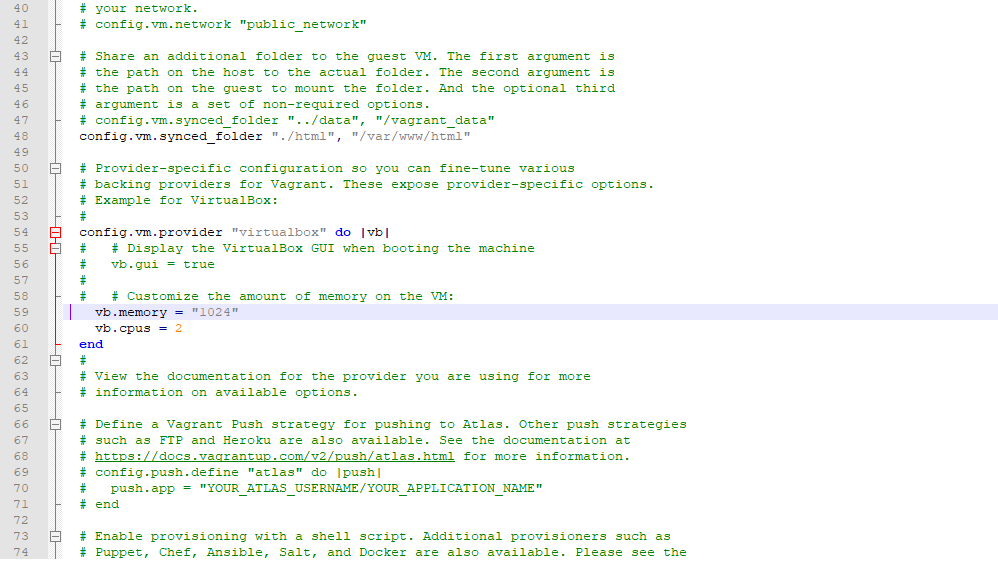
\includegraphics[width=13cm]{4-23.png}
\caption{Vagrantfile メモリ増設}\label{4-23}
\end{figure}

以上が終わったら,仮想マシンを起動し,ログインをする.これは4.3.3章に記述したとおりである.なお,初回であるため,時間がかかる.

vagrant up

vagrant ssh

\newpage

\subsection{pythonの導入}
wget https://www.python.org/ftp/python/3.4.3/Python-3.4.3.tgz

sudo apt install zlib-devel bzip2-devel openssl-devel ncurses-devel sqlite-devel readline-devel tk-devel

以上のコマンドを入力し実行する.そして,pythonと入力し,以下のような画面が出たら,Pythonがインストールできている.
\begin{figure}[htb]
\centering
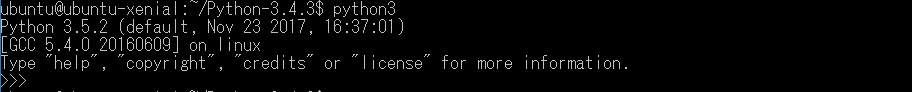
\includegraphics[width=13cm]{4-24.png}
\caption{Python導入}\label{4-24}
\end{figure}
\newpage

\subsection{MeCabの導入}
MeCabとは,オープンソースの形態素解析ツールである.

以下のコマンドでインストールを行こなう.

sudo apt install -y mecab mecab-ipadic-utf8 libmecab-dev

\begin{figure}[htb]
\centering
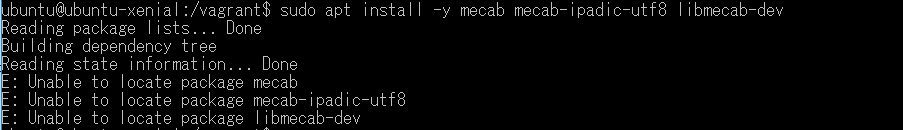
\includegraphics[width=13cm]{4-25.png}
\caption{MeCab導入}\label{4-25}
\end{figure}
\newpage

\subsection{gensimの導入}

Word2vec用ライブラリである,gensimをインストールする.下記コマンドによってインストールできる.

pip install gensim

\begin{figure}[htb]
\centering
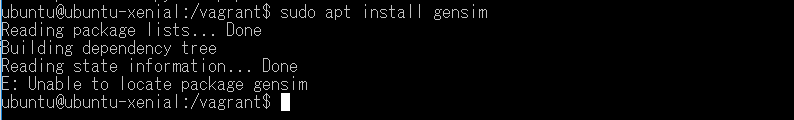
\includegraphics[width=13cm]{4-26.png}
\caption{gensim導入}\label{4-26}
\end{figure}
\newpage

\subsection{コーパスダウンロード}

本研究では,東北大学乾・岡崎研究所より提供されている「日本語Wikipediaエンティティベクトル」を使用し,研究を進める.

下記コマンドによって導入を行う.


cd /vagrant

wget http://www.cl.ecei.tohoku.ac.jp/~m-suzuki/jawiki\_vector/data/20170201.tar.bz2

tar xf 20170201.tar.bz2

以下のように何も出なければ成功である.

\begin{figure}[htb]
\centering
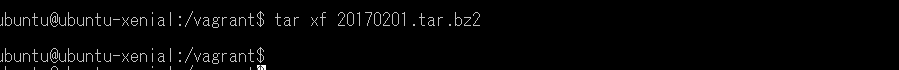
\includegraphics[width=13cm]{4-27.png}
\caption{コーパス導入}\label{4-27}
\end{figure}
\newpage

\section{Word2vec}

pythonとしてインタラクティブシェルを起動する.起動の仕方は以下の通りである.

python3 と入力する.

以下のようになれば起動完了である.ここでは,pythonを利用しての作業ができる.

\begin{figure}[htb]
\centering
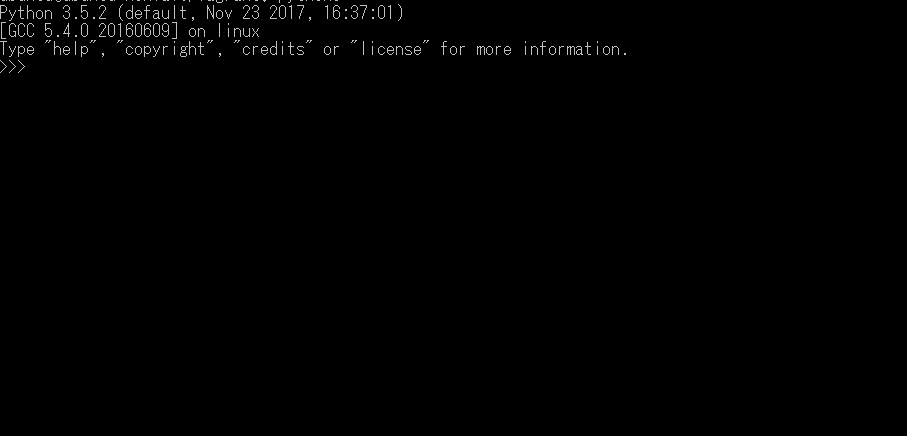
\includegraphics[width=13cm]{4-28.png}
\caption{Pythonインタラクティブシェル}\label{4-28}
\end{figure}
\newpage

Word2vecは単語をベクトルで表すことができ,さらに,算出したベクトルから,単語と単語の計算をすることができる.

例えば,「手帳」という単語のベクトルを表そうとすると,下記のようなコマンドを入力する.

import gensim

model = gensim.models.KeyedVectors.load\_word2vec\_format('entity\_vector/entity\_vector.model.bin', binary=True)

tmp = model['手帳']

print(tmp)

\begin{figure}[htb]
\centering
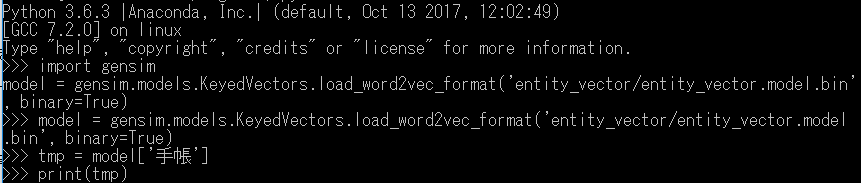
\includegraphics[width=13cm]{4-29.png}
\caption{「手帳」のベクトル}\label{4-29}
\end{figure}
\newpage

結果は下記のように表示される.

\begin{figure}[htb]
\centering
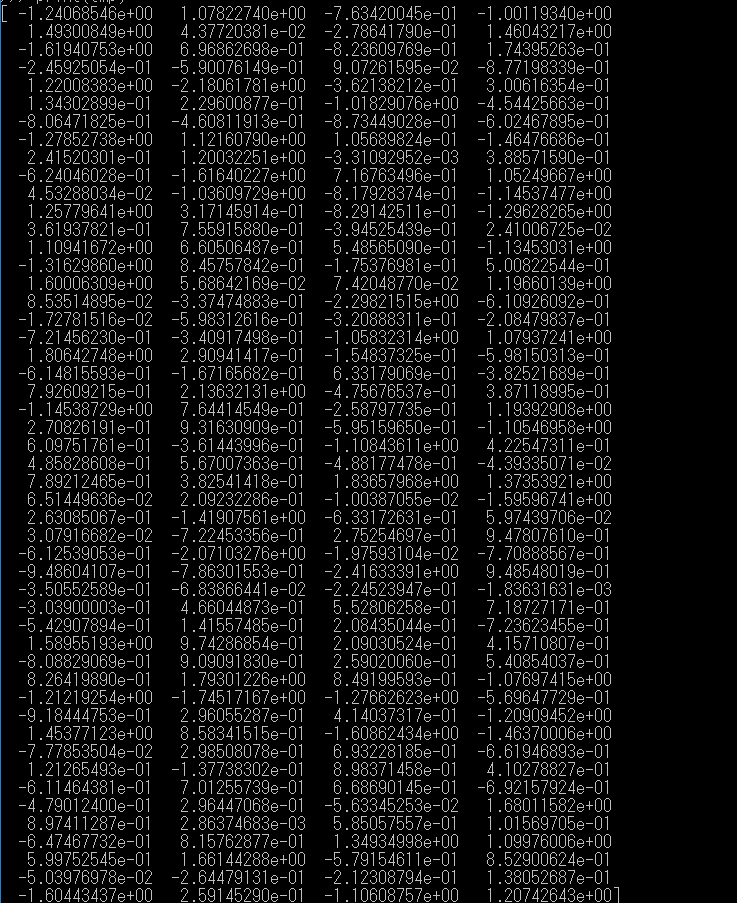
\includegraphics[width=13cm]{4-30.png}
\caption{「手帳」のベクトル 結果}\label{4-30}
\end{figure}
\newpage

\subsection{Rの導入}
R言語とは,統計解析やその結果をグラフィカルに表示するためのシステム「R」用の言語のことである.R言語は、AT\&Tベル研究所の研究者によって設計された統計処理言語であるS言語を元に設計されている.同じくAT\&Tベル研究所のが開発した「S言語」の実装系は商用版が知られているが,R言語はGNUプロジェクトによってオープンソースで提供されており,無償で利用することができる.R言語は,簡単なコ マンドによりいろいろな機能が実現できる.標準では用意されていない機能も比較的容易 に拡張できるメリットがある.

インストールは,chocolateyから行うことができる.

windowsの管理者権限のあるコマンドプロンプトを立ち上げ,以下のコマンドを入力する.

choco install r.project

\begin{figure}[htb]
\centering
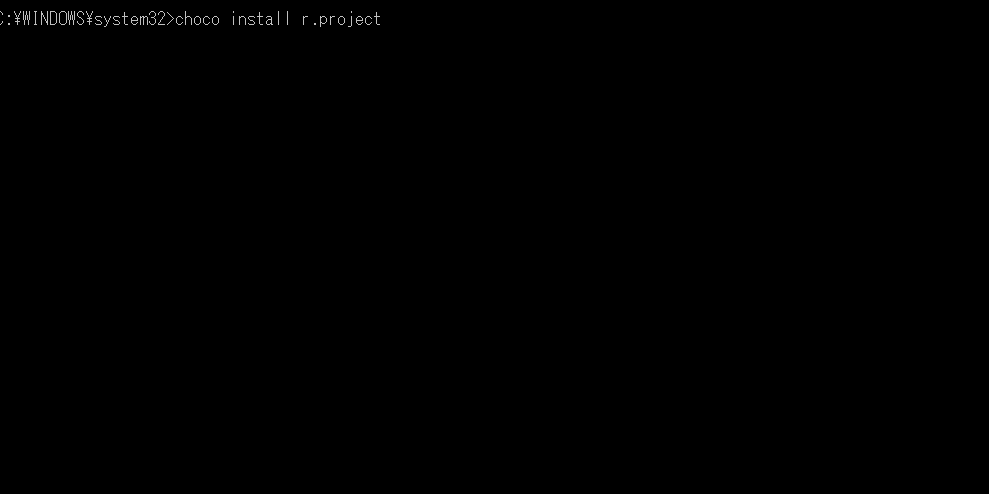
\includegraphics[width=13cm]{4-31.png}
\caption{R のインストール}\label{4-31}
\end{figure}
\newpage

次に,実際に本研究と同内容のword2vecの扱いをしていく.
大まかな流れとしては以下の通りである.
\begin{enumerate}
 \item 1文章ごとに区切る.
 \item タグ付けを行い,CSVファイルにまとめる.
 \item MeCabを利用し,分かち書き処理をさせる.
 \item ベクトル化する.
 \item 主成分分析を行う.
 \item 比較・考察を行う.
\end{enumerate}
\newpage

\subsection{解析対象文}

私自身の3年次の課題研究概要で書いた文章を例に手法を書く.解析対象文は以下のとおりである.

少子高齢化が進み,健康寿命が短くなっている現在,介護業界はこれから重要となり,需要も増加傾向にある業界である.実際に特別養護老人ホームの入所申込者数(待機者数)は09年~14年の5年間で10万人増加している.待機者数増加の要因として考えられるのは,1947年~1949年に生まれた団塊世代の人たちが徐々に介護サービスを必要としてきているからである.

介護職員は賃金,労働時間,体力的,精神的な負担が大きい.これらの要因から介護現場は厳しい労働環境であり,離職率が高い.さらに平成26年時点で介護分野における有効求人倍率が2倍を超えている状況であるため,増える介護の需要に介護職員の人数が追いついていないといえる.介護現場の人材不足を解消するには介護のオートメーション化や外国人労働者の雇用,介護職員の負担軽減が必要であると考えられる.

以上の2段落7文章である.
\newpage

この文章を解析用ファイルとして下図のようにCSVファイルにする.

タグAは1段落目を表し,タグBは2段落目を表している.

これを,仮に”01.csv”として保存する.
\begin{figure}[htb]
\centering
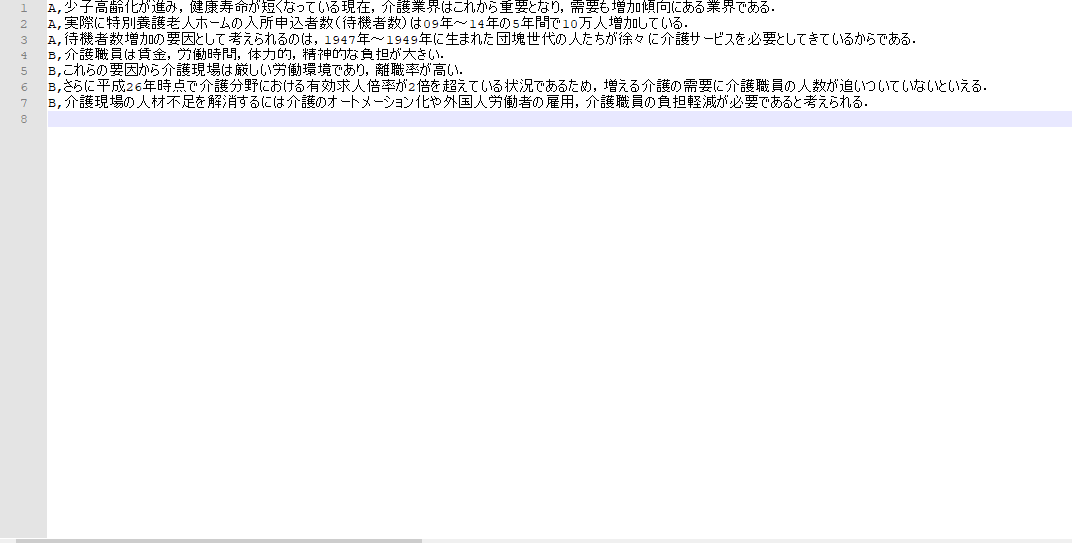
\includegraphics[width=13cm]{4-32.png}
\caption{解析前CSVファイル}\label{4-32}
\end{figure}
\newpage

保存が完了したら,vagrant上で分かち書き処理をし,ベクトル化処理をする.

下図のように何もエラーがでなければ成功である.

cat 01.csv | python s2v.py > 01vec.csv

\begin{figure}[htb]
\centering
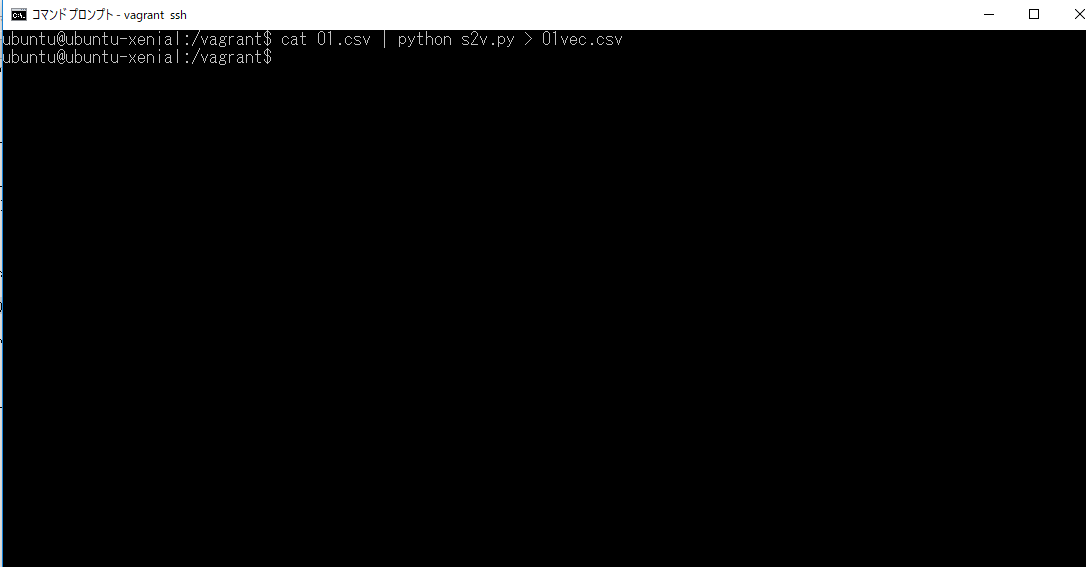
\includegraphics[width=13cm]{4-33.png}
\caption{ベクトル化}\label{4-33}
\end{figure}
\newpage

ベクトル化されたデータは,”01vec.csv”として同フォルダ内に保存されている.
\begin{figure}[htb]
\centering
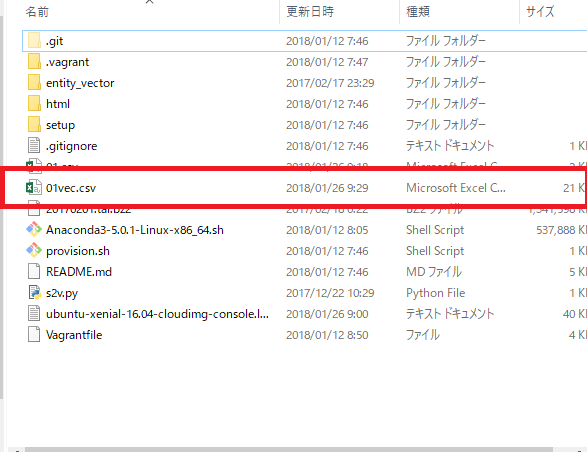
\includegraphics[width=13cm]{4-34.png}
\caption{ベクトルされたデータ}\label{4-34}
\end{figure}
\newpage

ベクトル化され出力されたデータの中身はこのようになっている.次にこの数値を主成分分析へかけていく.

\begin{figure}[htb]
\centering
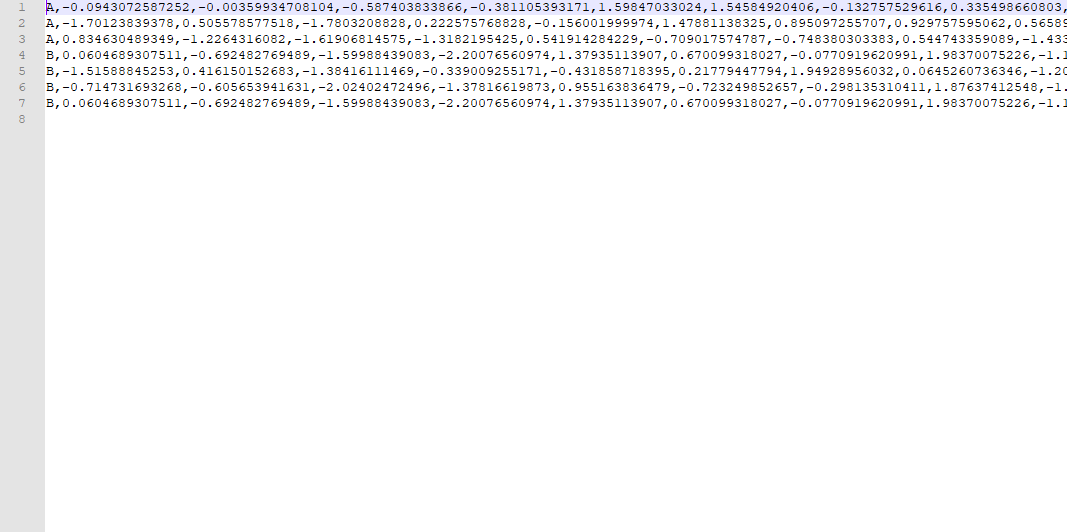
\includegraphics[width=13cm]{4-35.png}
\caption{01vec.csv}\label{4-35}
\end{figure}
\newpage

Rを起動し,きれいな描画のためのツールをインストールする.

コマンドは下記の通りである.

install.packages(”devtools”)

devtools::install\_github(”vqv/ggbiplot”)

下図のようにエラーが出なければインストール完了である.

\begin{figure}[htb]
\centering
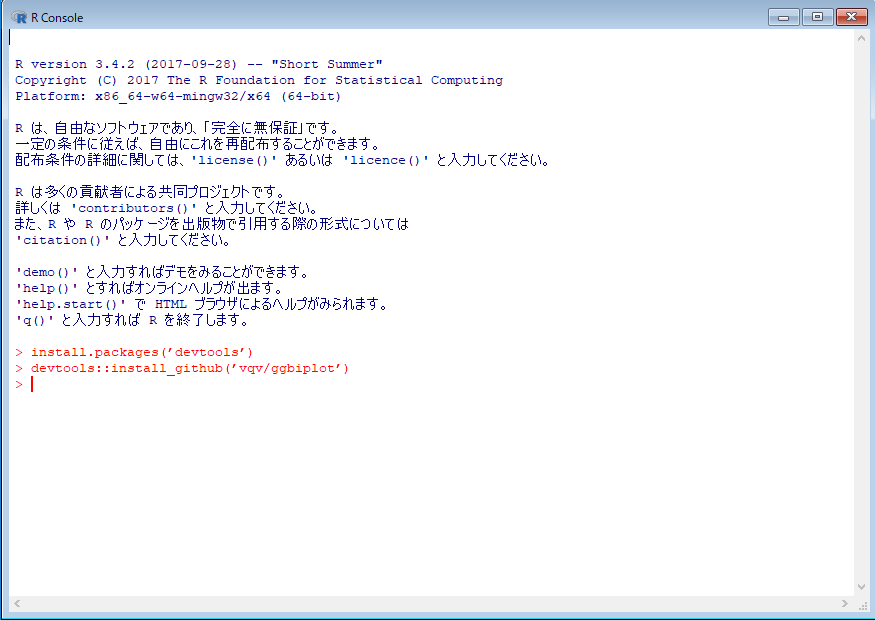
\includegraphics[width=13cm]{4-36.png}
\caption{きれいな描画のためのツール}\label{4-36}
\end{figure}
\newpage

続いて,主成分分析へ入る.

setwd('c:/vagrant/machine')\#作業ディレクトリの変更

myData <- read.csv('01vec.csv', head = F)

myResult <- prcomp(myData[, -1])\#主成分分析

library(ggbiplot)

ggbiplot(myResult, var.axes = F, groups = myData[, 1])

このコマンドを実行し,エラーが出なければ成功である.

\begin{figure}[htb]
\centering
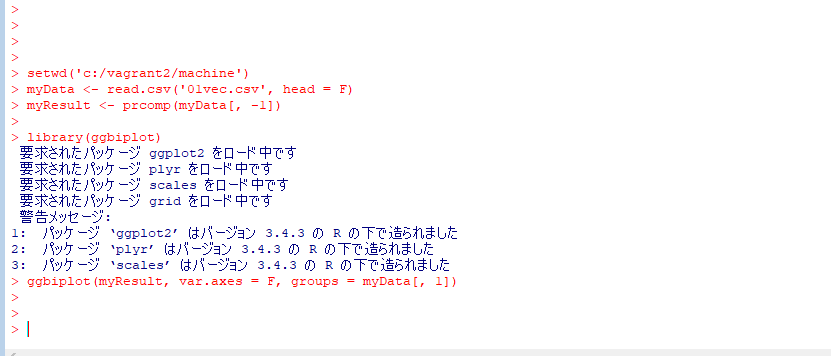
\includegraphics[width=13cm]{4-37.png}
\caption{Rで主成分分析}\label{4-37}
\end{figure}
\newpage

主成分分析の結果である. 
これを比較し,考察していく.

\begin{figure}[htb]
\centering
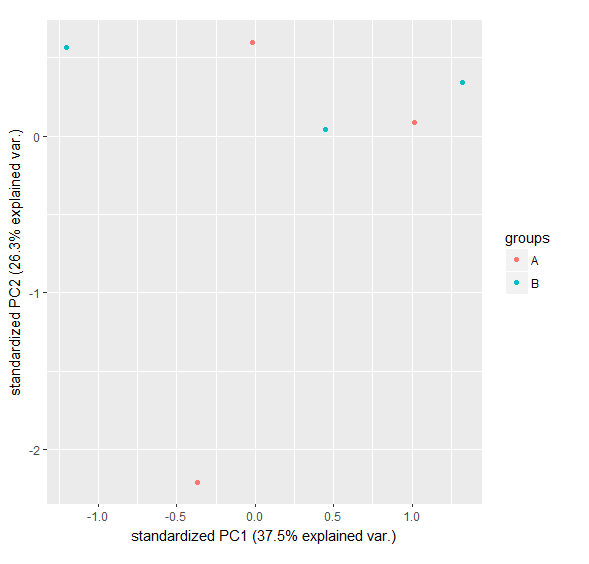
\includegraphics[width=13cm]{4-38.png}
\caption{主成分分析の結果}\label{4-38}
\end{figure}
\newpage

\chapter{結果}

word2vecを用い,数値的に文章構造の解析をした結果である.以下が解析対象文である.

少子高齢化が進み,健康寿命が短くなっている現在,介護業界はこれから重要となり,需要も増加傾向にある業界である.実際に特別養護老人ホームの入所申込者数(待機者数)は09年~14年の5年間で10万人増加している.待機者数増加の要因として考えられるのは,1947年~1949年に生まれた団塊世代の人たちが徐々に介護サービスを必要としてきているからである.

介護職員は賃金,労働時間,体力的,精神的な負担が大きい.これらの要因から介護現場は厳しい労働環境であり,離職率が高い.さらに平成26年時点で介護分野における有効求人倍率が2倍を超えている状況であるため,増える介護の需要に介護職員の人数が追いついていないといえる.介護現場の人材不足を解消するには介護のオートメーション化や外国人労働者の雇用,介護職員の負担軽減が必要であると考えられる.

ここまで解析対象文である.

\begin{figure}[htb]
\centering
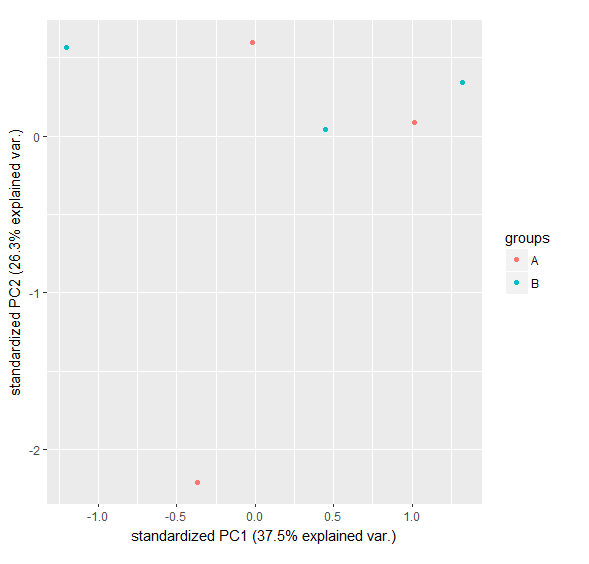
\includegraphics[width=13cm]{4-38.png}
\caption{主成分分析の結果}\label{4-38}
\end{figure}
\newpage

2つめの解析対象文章である.これは新聞記事である.

総務省が26日発表した2017年12月の全国消費者物価指数(CPI、2015年=100)は、値動きの大きな生鮮食品を除く総合指数が100.7と、前年同月比0.9%上昇した。プラスは12カ月連続。QUICKがまとめた市場予想の中央値(0.9%上昇)と同水準だった。ガソリンなどエネルギー価格上昇の影響が大きかった。

 生鮮食品を含む総合は101.2と1.0%上昇した。エネルギー価格上昇のほか、レタスなど葉物野菜の生育遅れと、ビールの値上がりなども押し上げ要因だった。一方で携帯電話料金や家電価格は下落しており、生鮮食品とエネルギーを除く総合は101.0と、0.3%の上昇にとどまった。

出典:2018/1/26 日本経済新聞

\begin{figure}[htb]
\centering
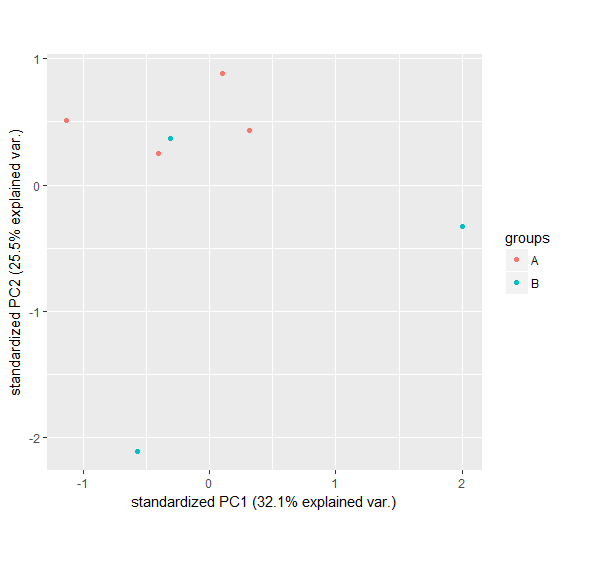
\includegraphics[width=13cm]{5-2.png}
\caption{分析結果}\label{5-2}
\end{figure}
\newpage

以下が3つ目の解析対象文である.

 内閣府は23日開いた経済財政諮問会議(議長・安倍晋三首相)で、「中長期の経済財政に関する試算」を提出した。試算では高成長シナリオで実質成長率が2020年度に1.5%、20年代前半から2%程度に達すると想定。国と地方の基礎的財政収支(プライマリーバランス、PB)の黒字化は昨年7月の試算より2年遅れて27年度になるとみている。

 内閣府は毎年、年初と夏に今後10年の成長率と財政の姿をまとめた中長期試算を公表する。今回は実質成長率が20年代前半に2%に達する「成長実現ケース」と、1%強の成長が続く「ベースラインケース」の2通りを示した。これまでも2通りのシナリオを公表してきたが、今回から高成長シナリオを過去の政策効果の実績を踏まえた現実的なものに変更した。
 
出典:2018/1/23 日本経済新聞

\begin{figure}[htb]
\centering
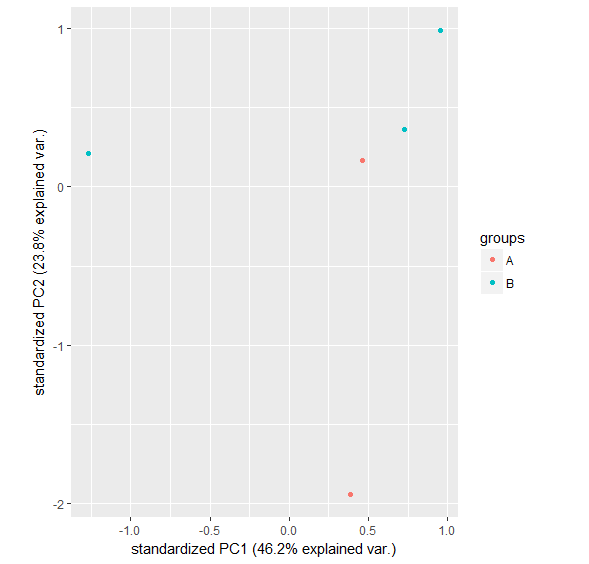
\includegraphics[width=13cm]{5-3.png}
\caption{分析結果}\label{5-3}
\end{figure}
\newpage

\chapter{考察}

このグラフからは,数値が散らばっているので,段落内で同じ話題が書かれているとは限らない.と考える事ができる.
\begin{figure}[htb]
\centering
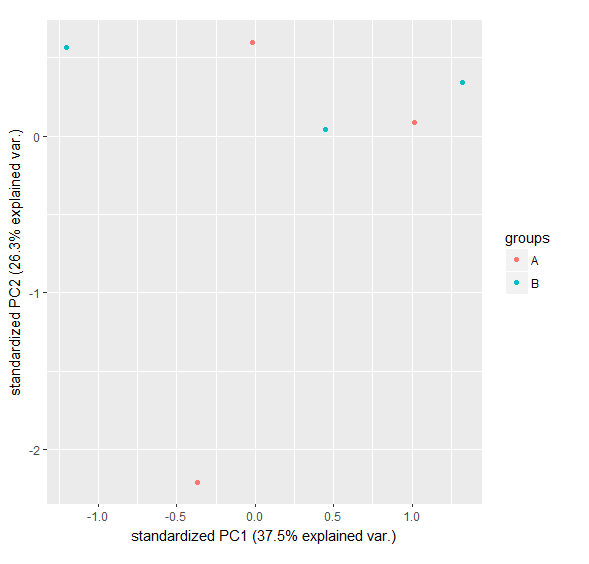
\includegraphics[width=13cm]{4-38.png}
\caption{主成分分析の結果}\label{4-38}
\end{figure}
\newpage

タグAの数値は割りと近い位置にプロットされており,話題の方向性が近いといえる.しかし,タグBはバラバラに散らばっているので方向性が近いとは言い難い.
\begin{figure}[htb]
\centering
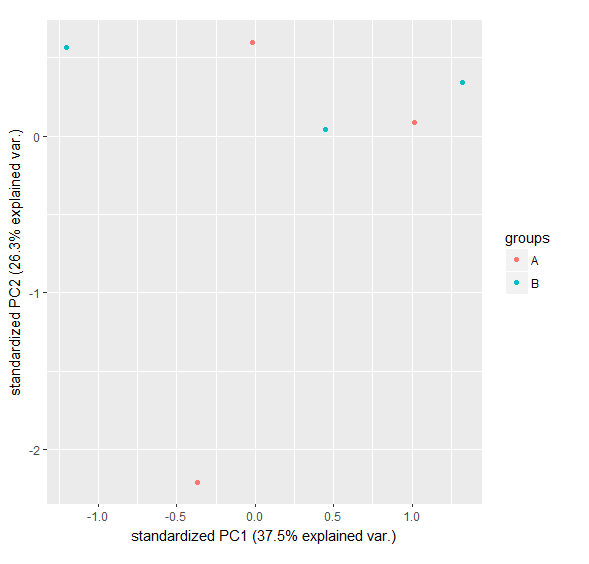
\includegraphics[width=13cm]{4-38.png}
\caption{主成分分析の結果}\label{4-38}
\end{figure}
\newpage

全体的に散らばっており,同じ話題の方向性とは言い難い.
\begin{figure}[htb]
\centering
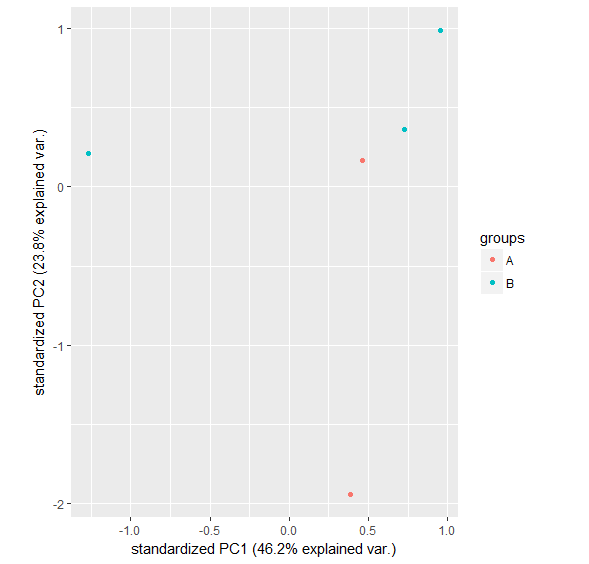
\includegraphics[width=13cm]{5-3.png}
\caption{分析結果}\label{5-3}
\end{figure}
\newpage


同段落内の文章は同じ話題でなければならないため,文章のベクトルも同じ方向性である必要がある.

分析結果では,一文章ごとの数値がグラフにプロットされている.このことから,文章の方向性が同じならば,タグAとタグBに対応する点がそれぞれ別々に集まることが期待される.

本研究での分析結果は,同段落内の文章にもかかわらず,それぞれのタグに対応する点が散らばって分布している.従って,解析対象文章の話題の方向性はバラバラであったと考えられる.

\chapter{結論}
今回の研究から,Word2vecを用いてベクトルへ変換した文章を定量的に検証することで,個人の主観による添削だけでなく,定量的な文章の添削を行うことが期待される.

\nocite{01}
\nocite{02}
\nocite{03}
\nocite{04}
\bibliographystyle{junsrt}
\bibliography{biblio}%「biblio.bib」というファイルが必要.

\chapter*{謝辞}\addcontentsline{toc}{chapter}{謝辞}
本研究を進めるにあたり,矢吹太朗准教授を始めとした矢吹研究室の先輩,同期,後輩の皆様には多くの時間を割いて頂き,様々なご助言をいただきました.この場を借りて深く御礼申し上げます.



\end{document}